\documentclass{beamer}

\mode<presentation> {
\usetheme[secheader]{Madrid}
\usecolortheme{seahorse}
\useinnertheme{circles}
}

\usepackage{graphicx} % Allows including images
\usepackage{booktabs} % Allows the use of \toprule, \midrule and \bottomrule in tables
\usepackage{tikz}
\usepackage{caption}
\usepackage{hyperref}

\setbeamerfont{section in sidebar}{size=\fontsize{5}{6}\selectfont}
\setbeamerfont{subsection in sidebar}{size=\fontsize{3}{5}\selectfont}
\setbeamerfont{subsubsection in sidebar}{size=\fontsize{2}{4}\selectfont}


%----------------------------------------------------------------------------------------
%	TITLE PAGE
%----------------------------------------------------------------------------------------

\makeatletter
%\patchcmd{\beamer@sectionintoc}{\vskip1.5em}{\vskip0.5em}{}{}
%\patchcmd{\beamer@subsectionintoc}{\vskip1.5em}{\vskip0.5em}{}{}
\makeatother



\title[Design of Everyday Things]{Design of Everyday Things} % The short title appears at the bottom of every slide, the full title is only on the title page

\author{Chaklam Silpasuwanchai} % Your name
\institute[AIT] % Your institution as it will appear on the bottom of every slide, may be shorthand to save space
{
Asian Institute of Technology \\ % Your institution for the title page
\medskip
\textit{chaklam@ait.asia} % Your email address
}
\date{} % Date, can be changed to a custom date

\AtBeginSection[]
{
\begin{frame}<beamer> 
\tableofcontents[currentsection]  % show TOC and highlight current section
\end{frame}
}

\begin{document}

\begin{frame}
\titlepage % Print the title page as the first slide
\end{frame}

\begin{frame}
\frametitle{Overview} % Table of contents slide, comment this block out to remove it
\footnotesize
\tableofcontents
 % Throughout your presentation, if you choose to use \section{} and \subsection{} commands, these will automatically be printed on this slide as an overview of your presentation
\end{frame}

%----------------------------------------------------------------------------------------
%	PRESENTATION SLIDES
%----------------------------------------------------------------------------------------

\begin{frame}
\frametitle{Sources} 
\begin{itemize}
	\item Norman, \textbf{The Design of Everyday Things}, Revised and Expanded ed. (2013)
	\item Shneiderman, \textbf{Designing the User Interfaces}, 6th ed. (2016). 
	\item Steve, \textbf{Don't Make Me Think: A Common Sense Approach to Web Usability}, 2nd ed. (2006). 
	\item Keith, Chapter 4, 6, 7, \textbf{Human Computer Interaction Course Notes}, Graz University (2017) - \url{https://courses.isds.tugraz.at/hci/hci.pdf}
	\item Jeff, \textbf{Designing with the Mind in Mind: Simple Guide to Understanding User Interface Design Guidelines}, 2nd ed. (2014).
\end{itemize}
\end{frame}


%------------------------------------------------
\section{Design of Everyday Things} % Sections can be created in order to organize your presentation into discrete blocks, all sections and subsections are automatically printed in the table of contents as an overview of the talk
%-----------------------------------------------

%\begin{frame}
%	\frametitle{Reminders}
%	\begin{itemize}
%		\item \textbf{Project leaders}:  You will receive feedback from your first draft  shortly.  Then please start your second round paper reading and check the deadline.
%		\item My feedback \textit{may} help you identify good topics.  \textbf{Your team needs to make the final judgement}.
%		\item Identify one or two \textbf{closest} work and identify their \textbf{limitations}.
%		\item In second round,  do the same thing, but with \textbf{any conferences/journals, NOT limited to CHI} and also with \textbf{any years} (but be smart).
%	\end{itemize}
%\end{frame}

%\begin{frame}
%\frametitle{Thinking Exercise}
%\begin{block}{Let's start with an activity}
%	Recall of two interactive products, one you enjoy using, and one so frustrating. \newline
%	What makes the differences?
%\end{block}
%\end{frame}
%
%\begin{frame}
%\frametitle{Usability vs. User Experience}
%\begin{itemize}
%	\item Usability
%	\begin{itemize}
%		\item \textbf{Effective} - does it achieve the goal?
%		\item \textbf{Efficient} - how much effort is required to achieve the goal?
%		\item \textbf{Safe} - how reliable and safe?
%		\item \textbf{Utility} - how convenient and versatile?
%		\item \textbf{Learnability} - can one learn your system?
%		\item \textbf{Memorability} - can one memorize commands?
%		\item \textbf{Accessibility} - can disabled people / elderly access your systems?
%	\end{itemize}
%	\item User Experience
%	\begin{itemize}
%		\item Reduce the negative aspects (e.g., frustration, annoyance)
%		\item Enhance the positive aspects (e.g., enjoyment, engagement)
%	\end{itemize}
%\end{itemize}
%\end{frame}
%
%\begin{frame}
%\frametitle{Usability vs. User Experience}
%Usability vs. User Experience
%\centering
%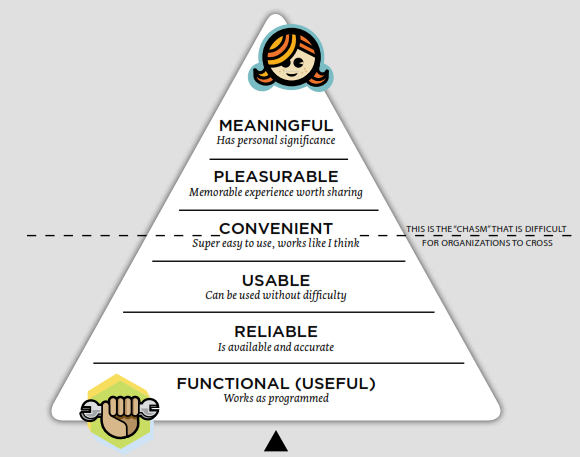
\includegraphics[width=.8\linewidth]{hierarchy}
%\end{frame}

\begin{frame}
\frametitle{Doors}
\centering
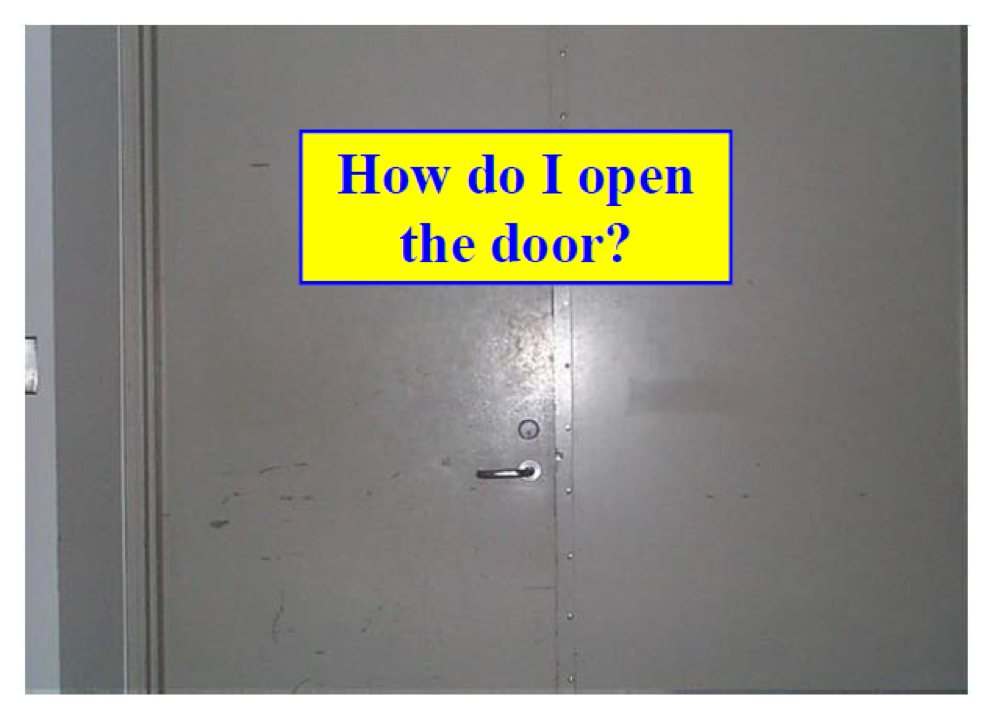
\includegraphics[width=0.8\linewidth]{door1}
\end{frame}

\begin{frame}
\frametitle{Doors}
\centering
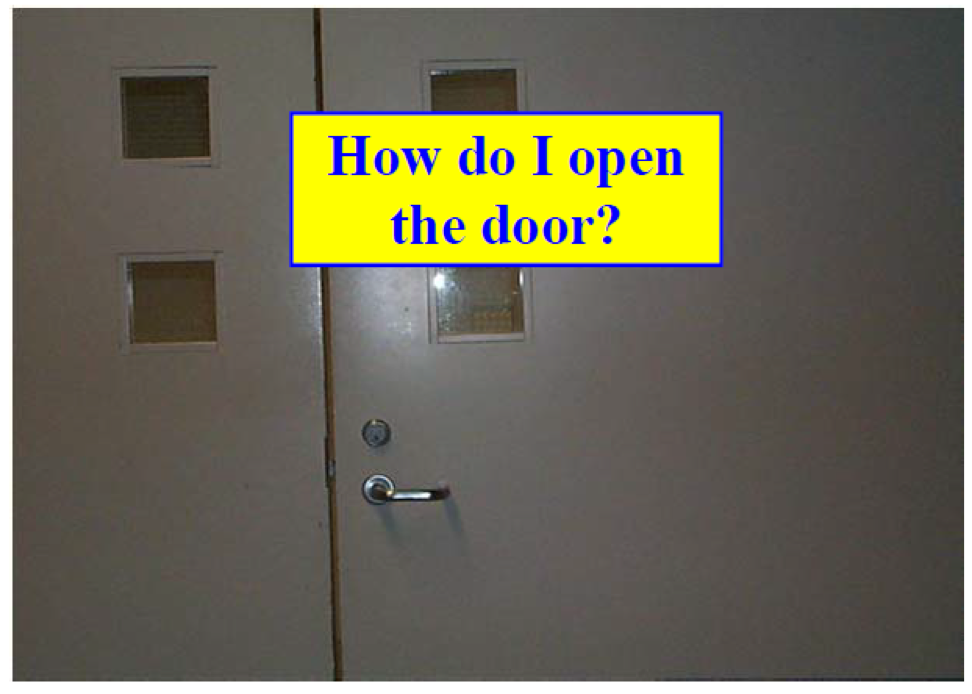
\includegraphics[width=0.8\linewidth]{door2}
\end{frame}

\begin{frame}
\frametitle{Doors}
\centering
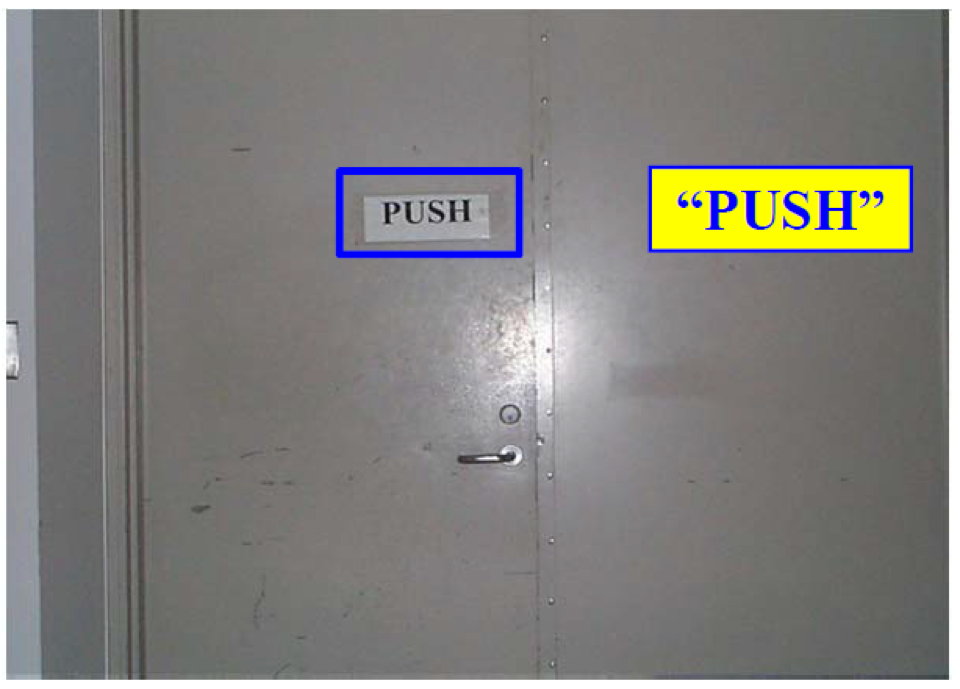
\includegraphics[width=0.8\linewidth]{door3}
\end{frame}

\begin{frame}
\frametitle{Doors}
\centering
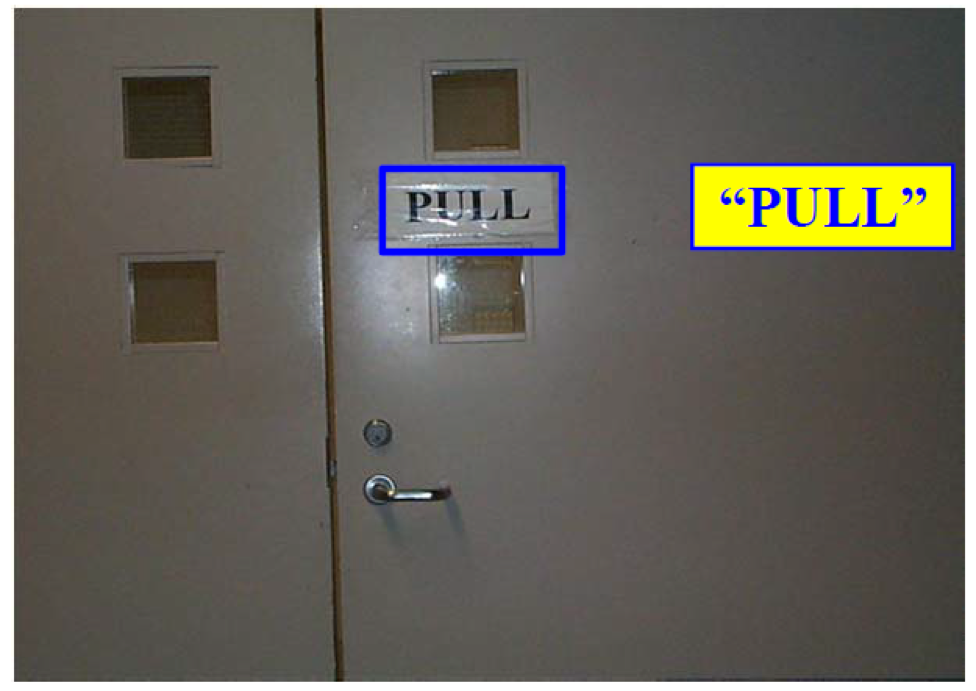
\includegraphics[width=0.8\linewidth]{door4}
\end{frame}

\begin{frame}
\frametitle{Doors}
\begin{itemize}
\item Good design is not vague.   It has only one \textbf{clear meaning}.
\item  Simple things \textit{should} be simple. \textbf{Instructions/explanations for simple things} are a \textbf{sign of failure}
\item Any better door?
\end{itemize}
\end{frame}

\begin{frame}
\frametitle{Doors}
\centering
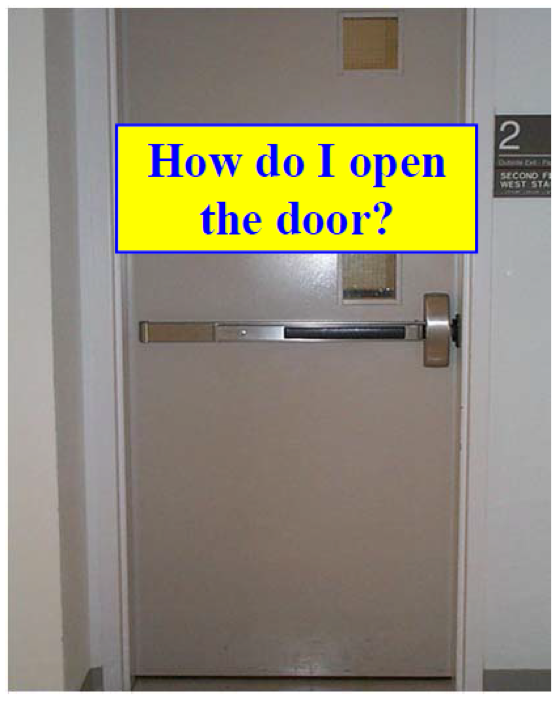
\includegraphics[width=.45\linewidth]{door5}
\end{frame}

\begin{frame}
\frametitle{Elevators}
\centering
%How many times - instead of opening, we close the elevator door?

\includegraphics[width=.7\linewidth]{elevator_bt}
\end{frame}

\begin{frame}
\frametitle{Elevators}
In a popular flanker test, the mean accuracy score 0.76 for incongruent trials and 0.98 for congruent trials
\newline \newline
\centering
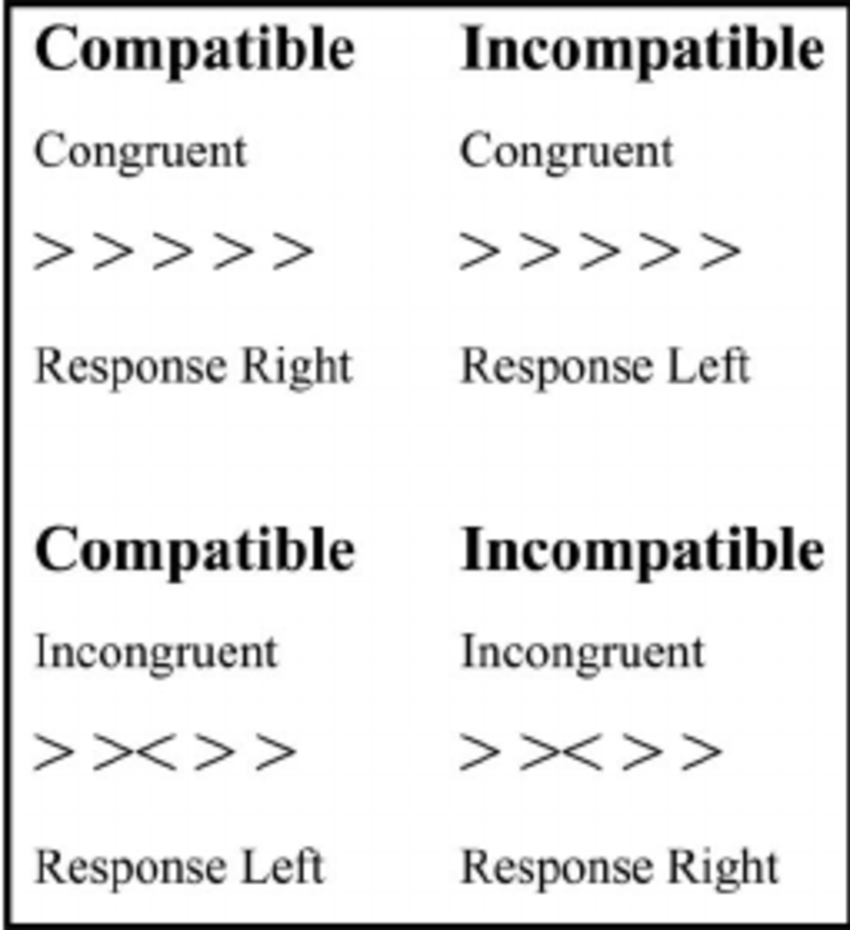
\includegraphics[width=.4\linewidth]{flanker}
\end{frame}


\begin{frame}
\frametitle{Projector}
%\begin{columns}[c] % The "c" option specifies centered vertical alignment while the "t" option is used for top vertical alignment
	
%	\column{.45\textwidth} % Left column and width
%	\centering
\centering
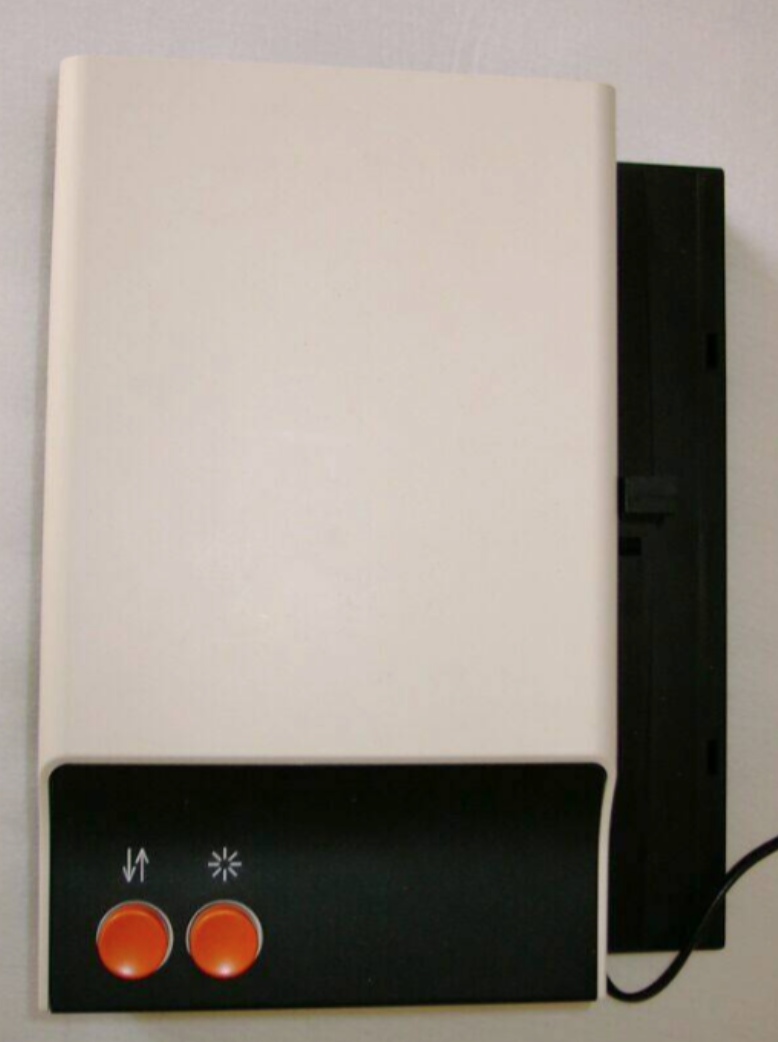
\includegraphics[width=0.45\linewidth]{zeiss}
%	Zeiss Slide Projector
	
%	\column{.55\textwidth} % Right column and width
%	\begin{itemize}
%		\item Hmm...how to use this machine?
%		\item What do you think?
%%		\item Only one button to control the slide advance
%%		\item During lectures, sometimes the slides go forwards, sometimes they go backwards
%%		\item If you can find an instruction manual; Short press = forward, long press = backward.
%%		\item What an elegant design!  two functions with one button (an engineer shouts!)
%%		\item But how should first time users know what to do?
%	\end{itemize}
%\end{columns}
\end{frame}

\begin{frame}
\frametitle{Toilet sign}
%\begin{columns}[c] % The "c" option specifies centered vertical alignment while the "t" option is used for top vertical alignment
%	
%	\column{.65\textwidth} % Left column and width
	\centering
	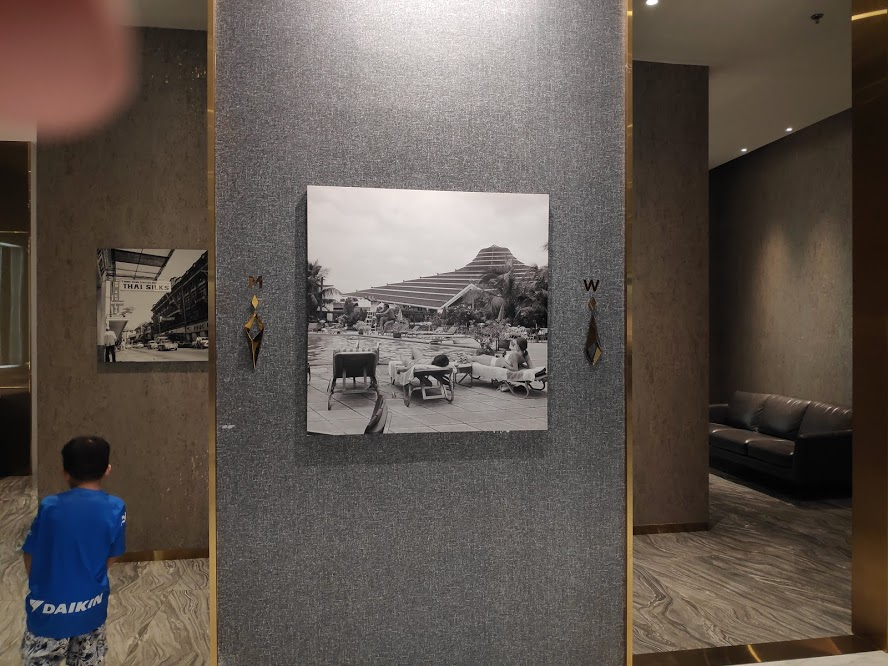
\includegraphics[width=0.8\linewidth]{toilet}
%	
%	\column{.35\textwidth} % Right column and width
%	\begin{itemize}
%		\item Took this picture at IconSiam
%		\item Which one is man and woman?
%		\item Minimalism or aesthetically pleasing are not design either!
%	\end{itemize}
%\end{columns}
\end{frame}

\begin{frame}
	\frametitle{Desk}
%	\begin{columns}[c] % The "c" option specifies centered vertical alignment while the "t" option is used for top vertical alignment
%		
%		\column{.65\textwidth} % Left column and width
		\centering
		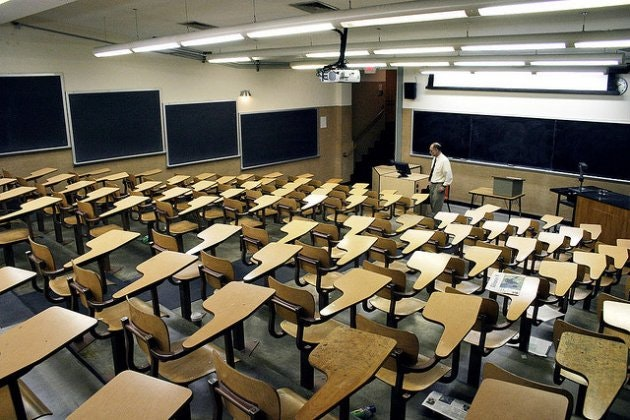
\includegraphics[width=0.8\linewidth]{desk}
%		
%		\column{.35\textwidth} % Right column and width
%		\begin{itemize}
%			\item Here, the desk is dominantly right-handed!
%		\end{itemize}
%	\end{columns}
\end{frame}

\begin{frame}
\frametitle{Mcdonald}
%\begin{columns}[c] % The "c" option specifies centered vertical alignment while the "t" option is used for top vertical alignment
%
%\column{.65\textwidth} % Left column and width
\centering
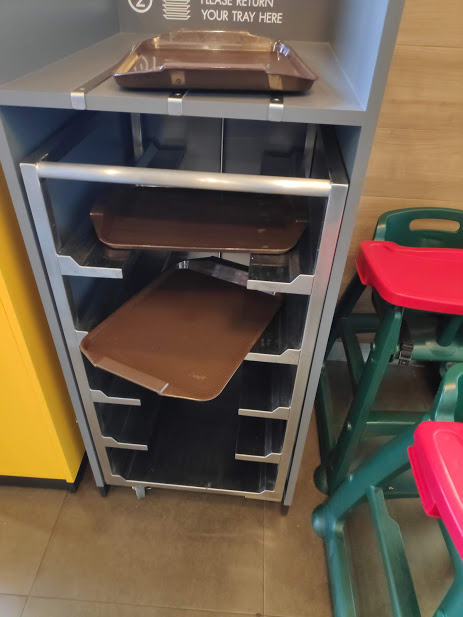
\includegraphics[width=0.45\linewidth]{mc}

%\column{.35\textwidth} % Right column and width
%\begin{itemize}
%	\item I have my lunch at a Mcdonald
%	\item I put the tray and it falls down
%	\item So how to design better?
%\end{itemize}
%\end{columns}
\end{frame}

\begin{frame}
\frametitle{Remote control}
\begin{columns}[c] % The "c" option specifies centered vertical alignment while the "t" option is used for top vertical alignment
	
	\column{.45\textwidth} % Left column and width
	\centering
	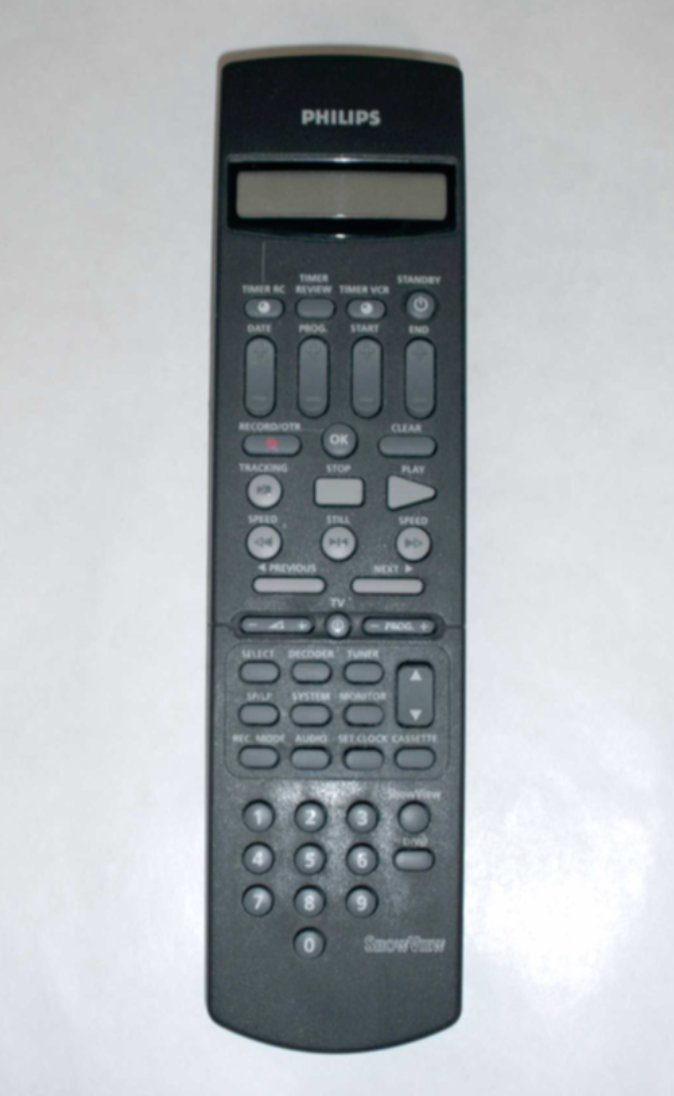
\includegraphics[width=0.8\linewidth]{remote}
	
	\column{.55\textwidth} % Right column and width
	\begin{itemize}
		\item Some of the buttons on a VCR remote control are easy to understand, but others are unfathomable without the instruction manual
		\item Remove buttons are not the solution either!  (this is in fact 90\% of what people will suggest which is wrong!  Why?)
		\item Better question is to ask how we can better support novice and expert users at the same time.
	\end{itemize}
\end{columns}
\end{frame}



\begin{frame}
\frametitle{TV gestures}
\centering
Never a commercial success.....why?
\newline \newline
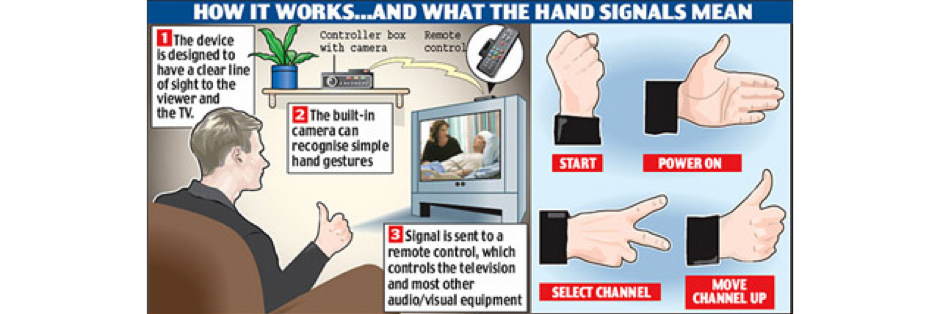
\includegraphics[width=1\linewidth]{tvgestures}
\end{frame}

\begin{frame}
\frametitle{List goes on....}
\begin{columns}[c] % The "c" option specifies centered vertical alignment while the "t" option is used for top vertical alignment
	
	\column{.45\textwidth} % Left column and width
	\centering
	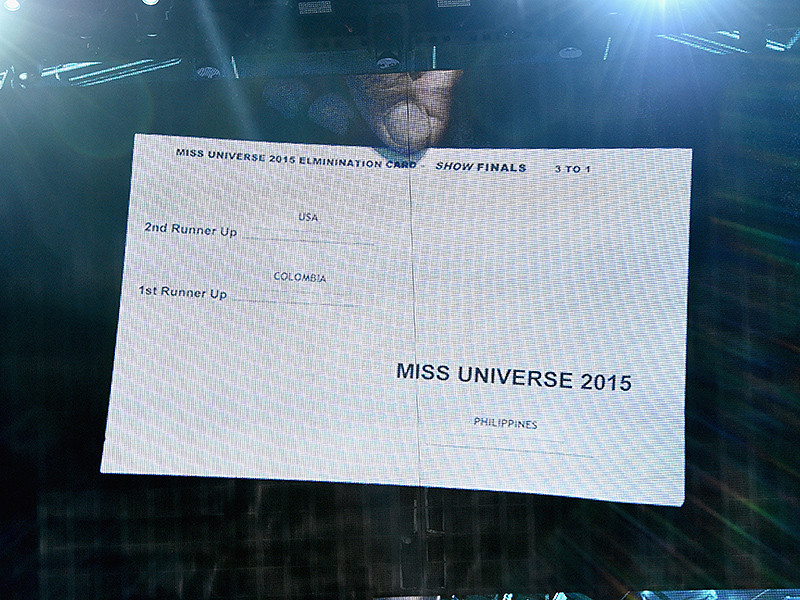
\includegraphics[width=1\linewidth]{universe}\newline
	
	\column{.55\textwidth} % Right column and width
	\begin{itemize}
		\item Do you remember \textbf{Miss Universe 2015} incident?
		\item How many times you or your acquaintances forgot to \textbf{withdraw your card from ATM}?
		\item How many times we forgot to \textbf{turn off the front lights of the car}?
		\item Have your mom/grandma go to a hotel and wonder \textbf{how to use the shower}?
	\end{itemize}
\end{columns}
\end{frame}

\begin{frame}
\frametitle{Stupid design is easy to avoid though}
\begin{columns}[c] % The "c" option specifies centered vertical alignment while the "t" option is used for top vertical alignment
	
	\column{.55\textwidth} % Left column and width
	\centering
	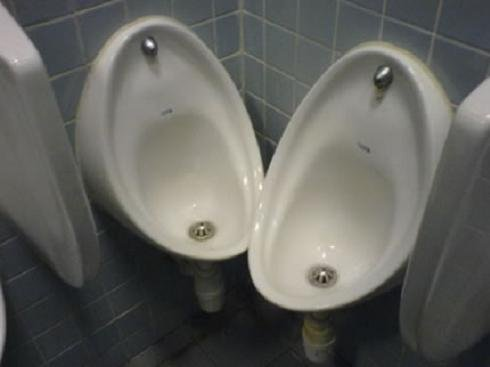
\includegraphics[width=1\linewidth]{toiletb}\newline
	
	\column{.45\textwidth} % Right column and width
	\begin{itemize}
		\item Of course, this class won't discuss these silly mistakes though %because they are just for the sake of joke.  Very few people really do that.  But this class gonna focus on "non-obvious" stuff
	\end{itemize}
\end{columns}
\end{frame}


\begin{frame}
\frametitle{Hmm...so why design goes wrong?}
\begin{itemize}
	\item Most engineers will often make the excuse of ``\textit{if the user read the instructions or manual}", or ``\textit{if the user click this before this}".  Preach \textbf{NEVER the fault of users, but of designers}
	\item Many design mistakes can be avoided by learning \textbf{design principles} %Most of the d 
	\item Engineering people usually \textbf{lack understanding of people}.  True? %The problem of engineers are that they are \textbf{too logical}, yet normal humans (even engineers themselves!) are quite diverse and usually less logical
	\item We are people ourselves, so we think \textbf{we understand people, but in fact, we don't}.  True? %\textbf{humans are amazingly complex}.  
\end{itemize}
\end{frame}


\begin{frame}
\frametitle{Why design is hard?}
\begin{itemize}
	\item Design is hard because of \textbf{tradeoffs}
	\begin{itemize}
		\item Top designers know what makes design good, but the problem is that you cannot always take all the good things
		\item Common \textbf{tradeoffs} - e.g., security vs convenience? familiarity vs. cool new experience? speed vs accuracy? customizability vs. learnability?
	\end{itemize}
	\item Design is hard because of \textbf{context}
	\begin{itemize}
		\item Context of use - which tasks the tools/systems are being used
		\item Expertise - novice vs. experts
		\item Cultural differences
		\item User groups (e.g., old vs. young, blind, female)
		\item Personal preferences!  
		\item Difficult to have \textbf{one-fits-all} solution
	\end{itemize}
\end{itemize}
\end{frame}

\begin{frame}
\frametitle{Why design is hard?}
\begin{itemize}
\item Design is hard because of \textbf{human nature}
\begin{itemize}
	\item Human \textbf{perception} is flawed
	\item Human \textbf{attention span} is limited
	\item Users does not like to \textbf{memorize}, nor \textbf{read}, nor \textbf{think}
	\item Users are \textbf{impatient}
	\item Humans are \textbf{NOT rational}
\end{itemize}
\end{itemize}
\begin{itemize}
\item Design is hard because of \textbf{engineer nature}
\begin{itemize}
	\item Engineer usually assumes users are same as him/her
	\item Engineer usually interested in solving technical challenge
	\item Engineers make stuff that only make sense to technical people
	\item Engineers make stuffs that usually are very logical and rational, which most users (could be engineers) are not
\end{itemize}
\end{itemize}
\end{frame}

\begin{frame}
\frametitle{What are some ways out?}
\begin{itemize}
	\item Understand people \textbf{expectations} and \textbf{knowledge}; they are not necessarily like you
	\item \textbf{Don't assume} people will read, learn, think, or care about your system
	\item Remember \textbf{diversity} - aged, blind, left-handed, experienced, does not know English etc.
	\item  \textbf{Rapid prototyping and failure}
	\item \textbf{Interview} but NOT follow
	\item NOT making it \textbf{simpler} nor \textbf{minimal} nor \textbf{ looking/feeling good},  they are secondary.  Primary is about \textbf{reaching the goal effectively and efficiently}
	\item Do \textbf{quantitative} user evaluation; don't argue
	\item Use good \textbf{design principles}
\end{itemize}
\end{frame}

%\begin{frame}
%\begin{center} 
%\usebeamerfont*{frametitle} \usebeamercolor[fg]{frametitle}  5-mins break 
%\end{center}
%\end{frame}

%\begin{frame}
%\frametitle{Fundamental Principles of Interaction}
%\begin{itemize}
%	\item Great designers produce \textbf{pleasurable experiences}.  But engineers tend not to like this word, it is too \textit{subjective}
%	\item When things \textit{work}, and users understand what it \textit{means}, it can lead to a feeling of control, of mastery, and of satisfaction.   \textbf{Cognition} and \textbf{emotion} are tightly intertwined, thus designers need to design with both in mind
%	\item Cognition \textbf{make sense} of the world; provide understanding, emotion \textbf{assigns value}, provides value judgments
%	\item When users interact with a product, they need to figure out how to work it, how it works, and what operations are possible.  This leads to one key principle: \textbf{discoverability}.
%	\item Discoverability results from application of \textbf{six principles}: \textit{affordances}, \textit{signifiers}, \textit{constraints}, \textit{mappings}, \textit{feedback}, and \textit{conceptual model}
%\end{itemize}
%\end{frame}


\section{Design Principles}

\subsection{Affordance}

\begin{frame}
\frametitle{Affordance}
\begin{itemize}
	\item When we see a glass, we know we need to hold it.  When we see a knob, we know we need to turn it.  The key principle here is \textbf{affordances}
	\item Affordance refers to the \textbf{relationship} between a physical object and a person.  A chair \textit{affords} support and, therefore, \textit{affords} sitting.  
	\item The notion of affordance comes with J. J. Gibson, an eminent psychologist who studied human perception.  He argued that the world contained \textbf{clues} what to do, and he called them \textbf{direct perception}.  In addition, he claimed that physical objects conveyed what actions are possible, which he named ``affordance"
\end{itemize}
\end{frame}

\begin{frame}
\frametitle{Affordance}
\centering
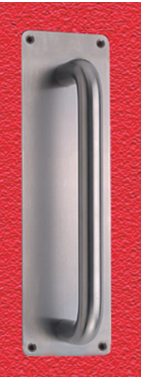
\includegraphics[width=0.2\linewidth]{affordance1}
\end{frame}

\begin{frame}
\frametitle{Affordance}
\centering

\includegraphics[width=0.8\linewidth]{affordance2}
\end{frame}

\begin{frame}
\frametitle{Affordance}
\centering
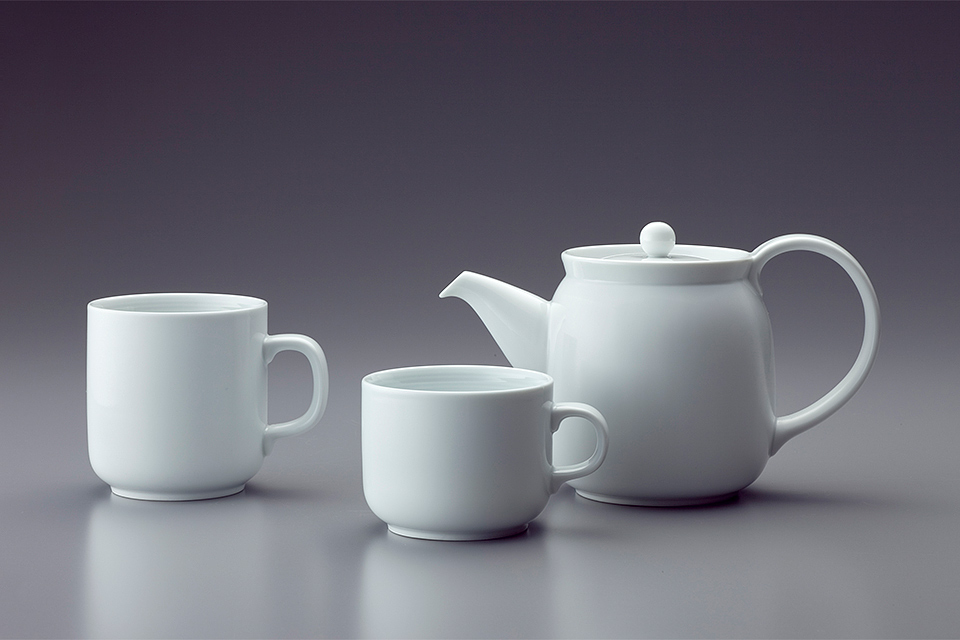
\includegraphics[width=0.8\linewidth]{affordance3}
\end{frame}

\begin{frame}
\frametitle{Affordance}
\centering
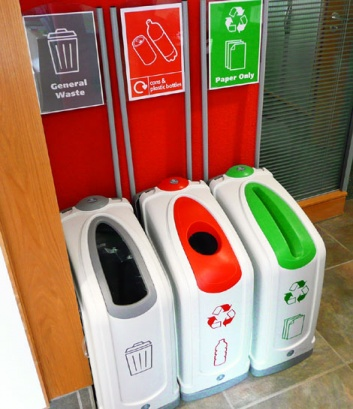
\includegraphics[width=0.5\linewidth]{affordance4}
\end{frame}

\begin{frame}
	\frametitle{Affordance}
	\centering
	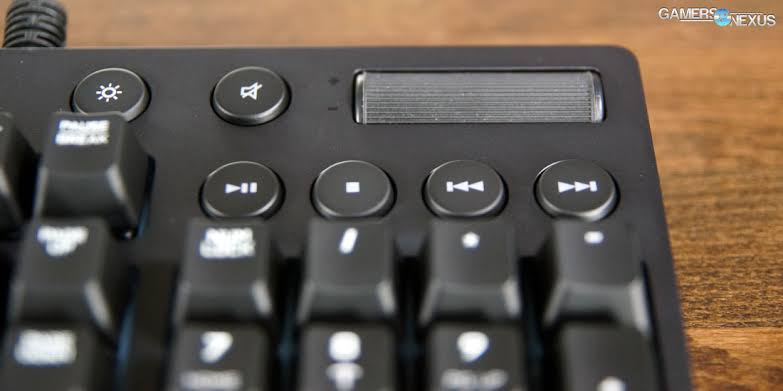
\includegraphics[width=0.8\linewidth]{orion}
\end{frame}

%\begin{frame}
%\frametitle{Affordance}
%	
%	Many affordances here.  What is good for controlling fan speed?  Which is good for turning on/off lights?  Which is good for adjusting stove heat?
%	
%	\centering
%	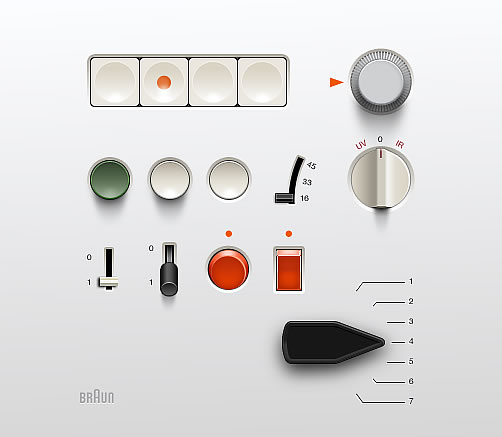
\includegraphics[width=0.5\linewidth]{affordance-activity}
%
%\end{frame}

\begin{frame}
\frametitle{Lack of affordance}
\centering
\begin{figure}
	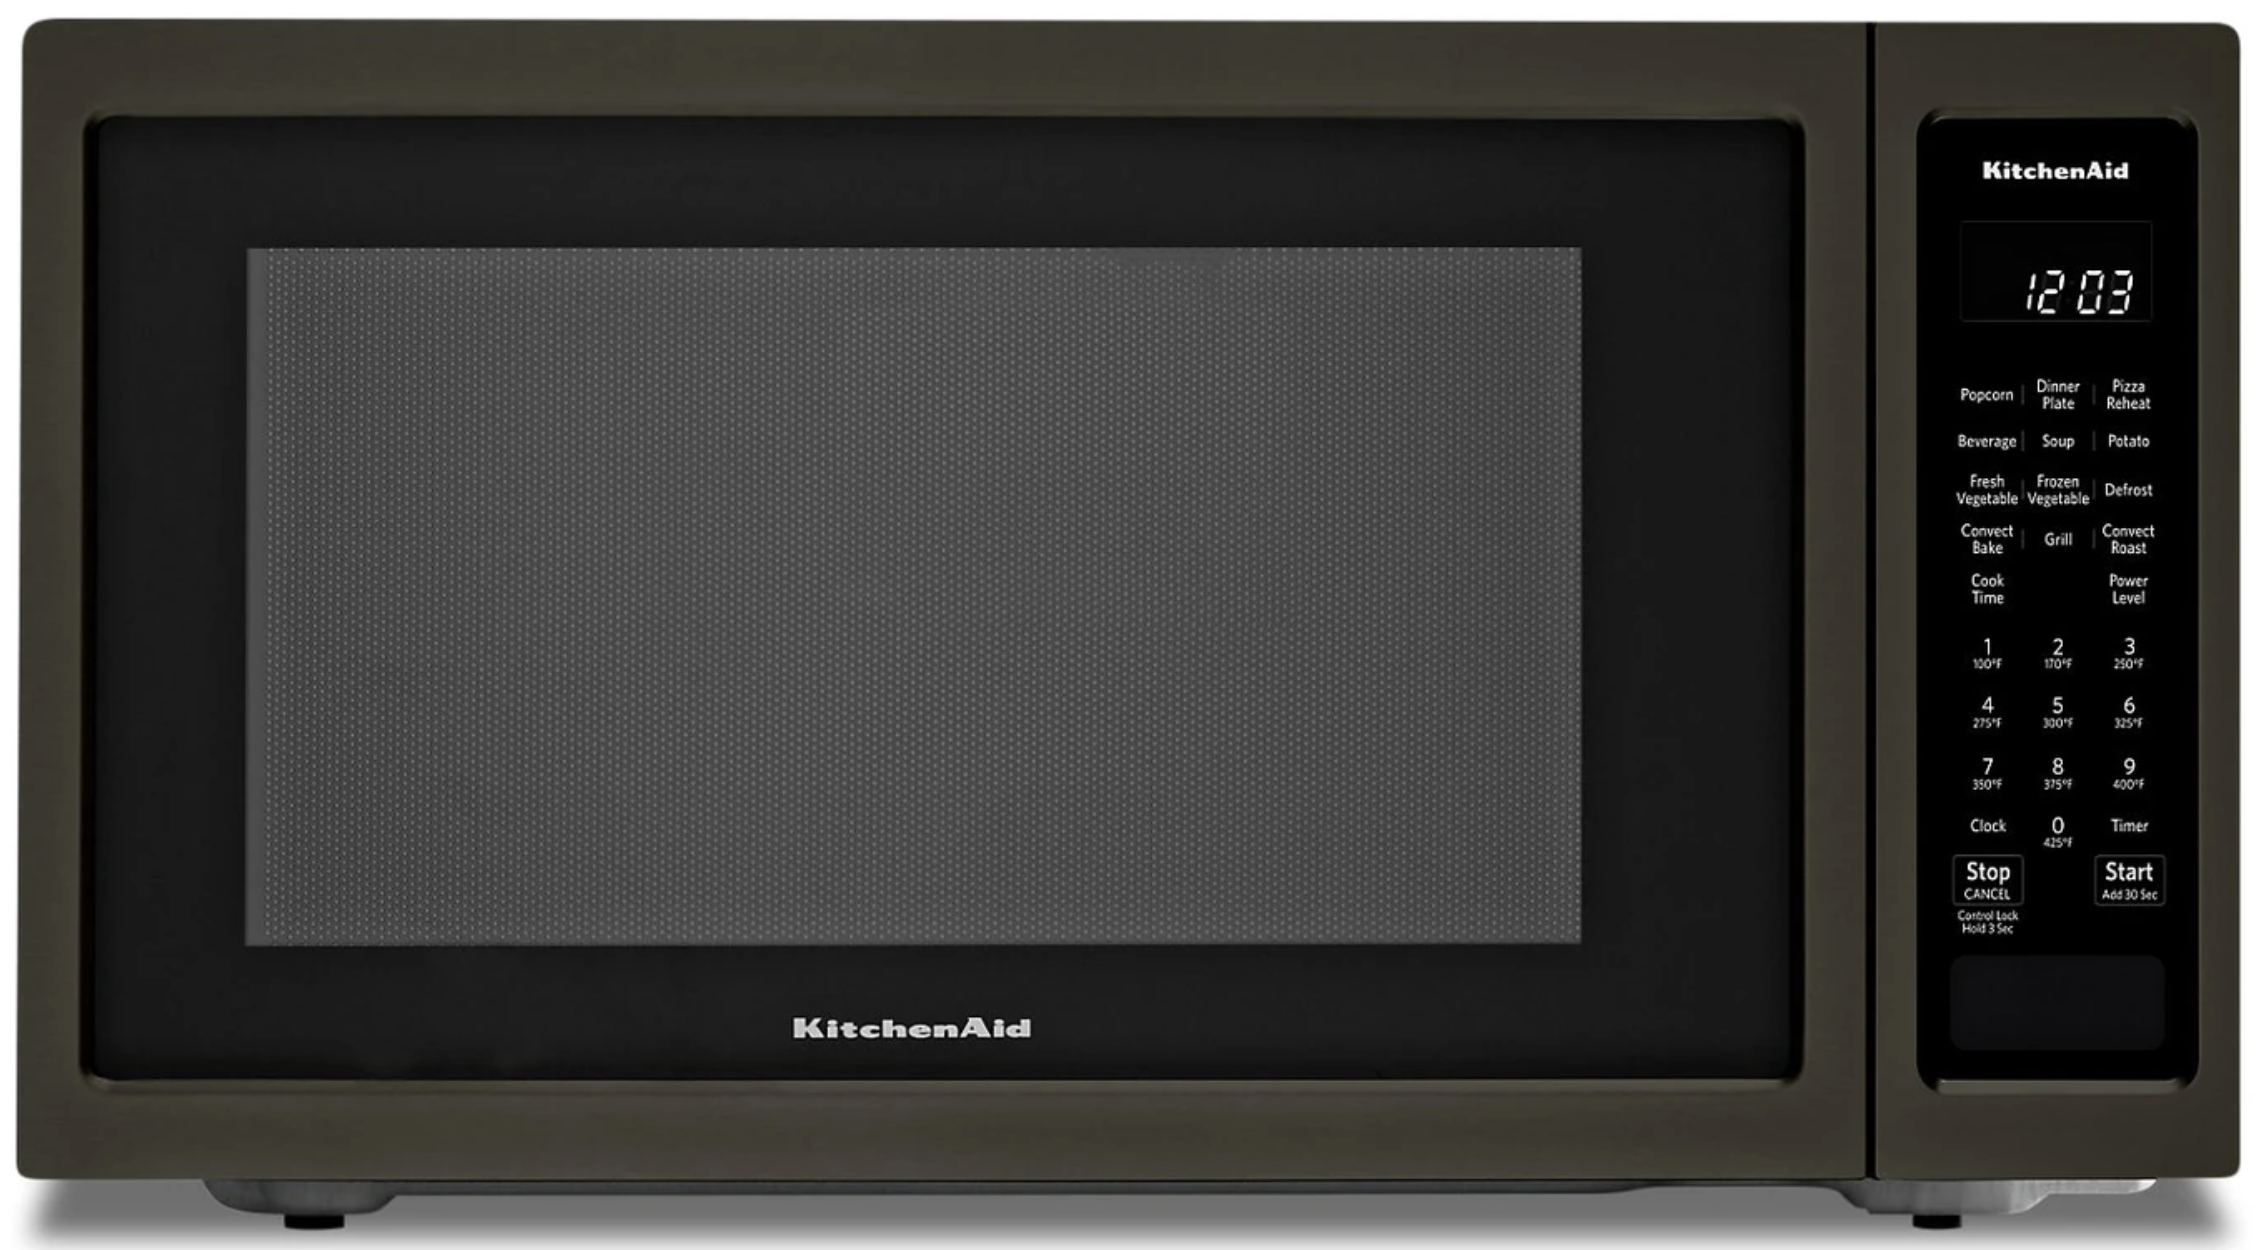
\includegraphics[width=0.7\linewidth]{microwave}
	\caption{Not sure how to open?}
\end{figure}
\end{frame}

\begin{frame}
	\frametitle{Lack of affordance}
	\centering
	\begin{figure}
		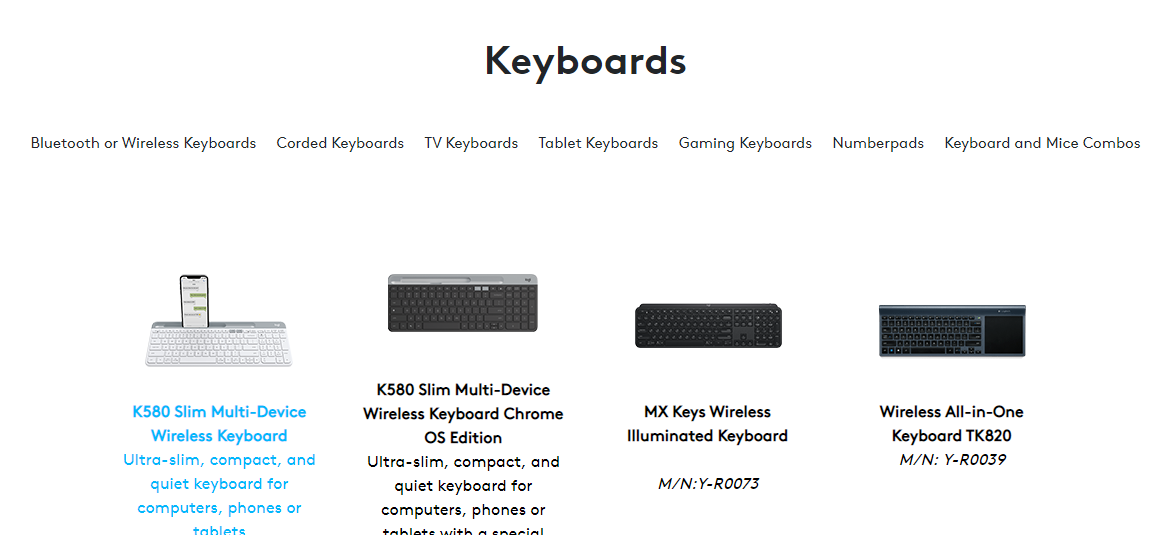
\includegraphics[width=0.9\linewidth]{clickable}
		\caption{Clickable?}
	\end{figure}
\end{frame}

\begin{frame}
\frametitle{Bad affordance}
\centering
Bad affordance also exists!  How many times did your family members put something on top of this similar machine?
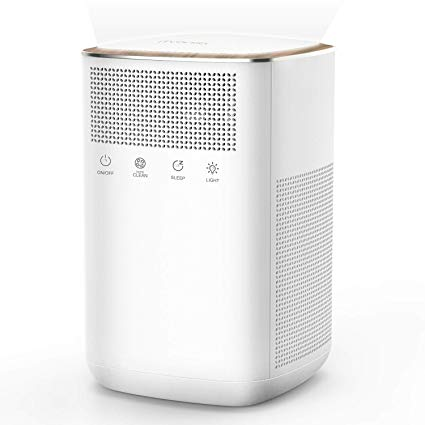
\includegraphics[width=0.5\linewidth]{badaffordance1}
\end{frame}
%
%\subsection{Signifiers}
%
%\begin{frame}
%\frametitle{Signifiers}
%\begin{itemize}
%	\item \textbf{Affordance} is about \textit{what} actions are possible, \textbf{signifiers} communicate \textit{where} the action should take place.  Both are needed
%	\item People need some way of understanding, some \textit{sign} of what it is for, what is happening, and what the alternative actions are.   Designers need to provide these clues
%	\item Signifiers refer to any \textbf{mark} or \textbf{sound}, any perceivable \textbf{indicator} that communicates appropriate behavior to a person
%	\item It can be \textbf{deliberate}, such like the sign PUSH on a door, can be \textbf{unintentional}, such as visible trail made by previous people walking or a bookmark telling how much of the book remains
%\end{itemize}
%\end{frame}

\begin{frame}
\frametitle{Affordance but lack of signifiers}
\centering
\begin{figure}
	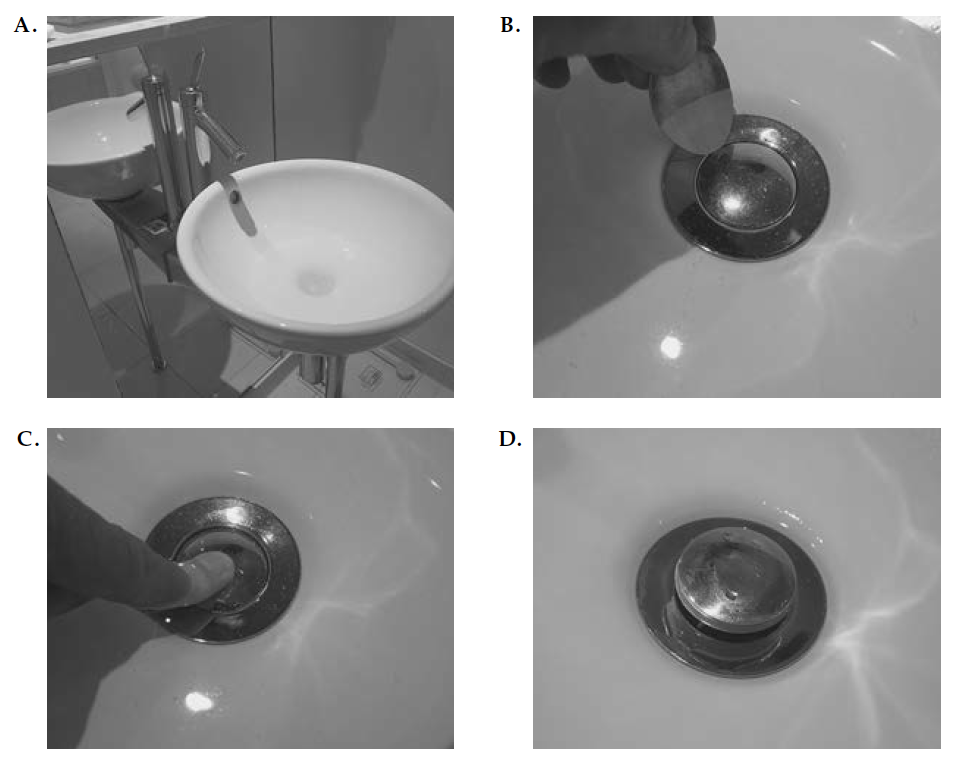
\includegraphics[width=0.65\linewidth]{sink}
	\caption{Source: Fg 1.4 (Norman) - Not sure how to take out!}
\end{figure}
\end{frame}
%
%\begin{frame}
%\frametitle{Signifiers vs. Affordances}
%\begin{itemize}
%	\item \textbf{Affordances} reveal what an object can do.  Yet, what an object can do is \textbf{only revealed by a user}.  Therefore, an affordance is what an object can do based on \textbf{interaction}.  An affordance can be obvious or hidden.
%	\begin{itemize}
%		\item A chair reveal its affordance by mirroring the shape of a body and communicates its intent: to be sat on
%		\item A chair also has hidden affordance, that is, chair can be use to reach a book, or move to other place
%	\end{itemize}
%	\item \textbf{Signifier} \textit{clarifies} an affordance.  It \textbf{bridges the gap} between truth (real affordance) and perception (perceived affordances). Signifier can be subtle or obvious.
%	\begin{itemize}
%		\item Some chairs have seats that are concave, shaped like a pair of butt cheeks, this design is subtle but acts as a signifier of the object's purpose
%		\item A door may have a slot, indicating that you probably can put something in.  A sign \textit{Mail} clarifies the purpose.
%		\item For accidental signifier, when you go to train platform and it's empty, it accidentally signifies that the train just left
%	\end{itemize}
%\end{itemize}
%\end{frame}
%
%\begin{frame}
%\frametitle{Signifiers vs. Affordances}
%\begin{itemize}
%	\item Signifier without affordance is a \textbf{mistake} (a door sign with a PUSH but with no real affordance).  But affordance can exist without signifiers.
%	\item Key point is to \textbf{introduce signifiers to make affordance visible}
%\end{itemize}
%\end{frame}


\subsection{Constraints}
\begin{frame}
\frametitle{Constraints}
\begin{itemize}
	\item Constraints is about \textbf{limiting what user can do}.  Why it is good?
	\item By \textbf{limiting users' options}, user has a better idea what to do
	\item \textbf{Lower} the chance for errors
	\item Humans also feel good when they see \textbf{limited }choices
\end{itemize}
\end{frame}

%\begin{frame}
%\frametitle{Physical, Cultural, Semantic, and Logical}
%\begin{itemize}
%	\item \textbf{Physical}: constrain possible operations.   Lego, for example.
%	\item \textbf{Cultural}: set of \textbf{acceptable action}s in society.  Red light is danger is US, death in Egypt, life in India, and happiness in China.   Down is off for US, but opposite for Britain.   Anti-clockwise is water on for US, but opposite for Britain
%	\item \textbf{Semantic}: constraints by \textbf{meaning}.  Rider sits only facing front, for example
%	\item \textbf{Logical}: constraints by logical or spatial relationships - similar to natural mappings
%\end{itemize}
%\end{frame}

\begin{frame}
\frametitle{Constraints}
\centering
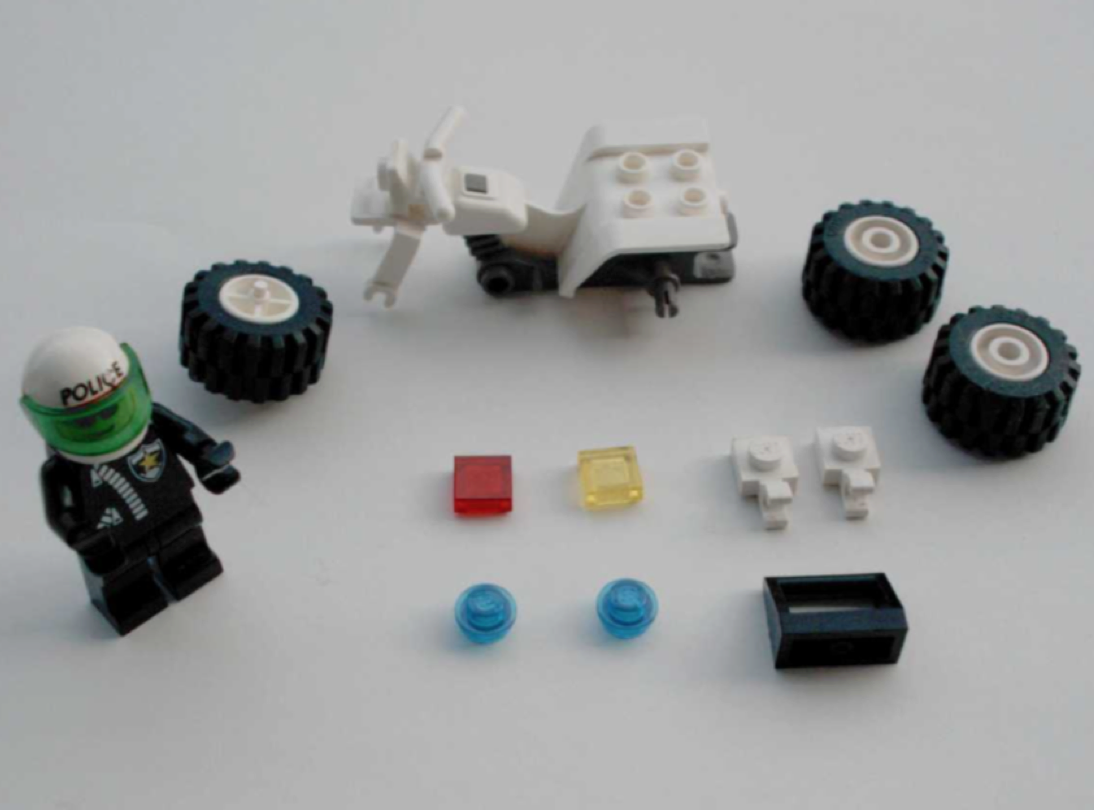
\includegraphics[width=0.50\linewidth]{lego1}
\begin{itemize}
\item Motorbike toy with 12 parts. Constraints make its construction simple, even for adults!
\begin{itemize}
	\item \textit{Physical}: Front wheel only fits in one place
	\item \textit{Semantic}: The rider sits on the seat facing forward
	\item \textit{Cultural}: Red is a rear light, yellow a front light
	\item \textit{Logical}: Two blue lights, two white pieces, go together
\end{itemize}
\end{itemize}
\end{frame}

\begin{frame}
\frametitle{Constraints}
\centering
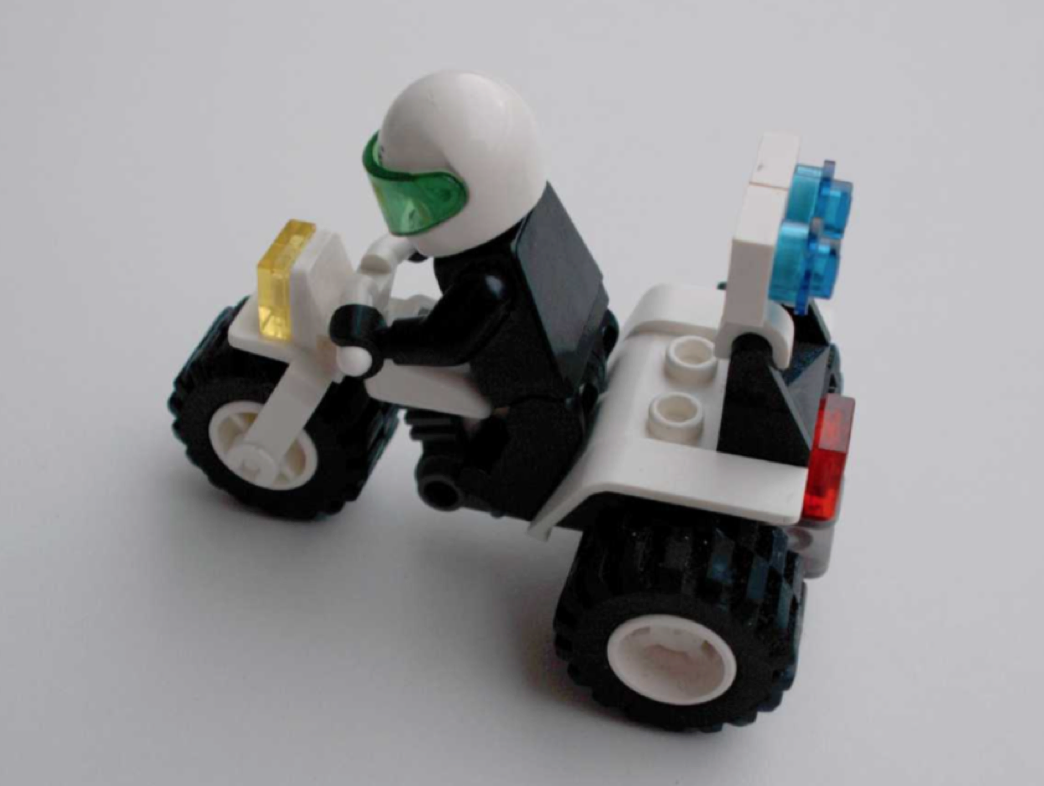
\includegraphics[width=0.7\linewidth]{lego2}
\end{frame}

\begin{frame}
\frametitle{Constraints}
\centering
\begin{figure}
	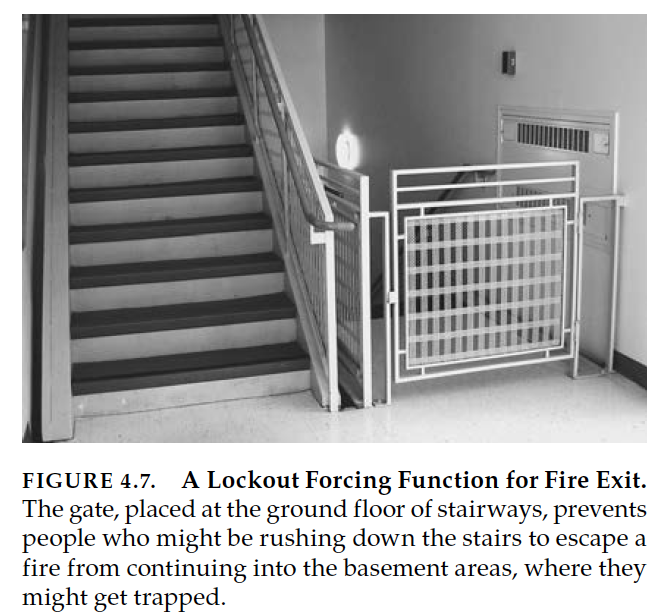
\includegraphics[width=0.6\linewidth]{force2}
	\caption{Source: Fg 4.7 (Norman)}
\end{figure}
\end{frame}

\begin{frame}
\frametitle{Constraints}
\centering
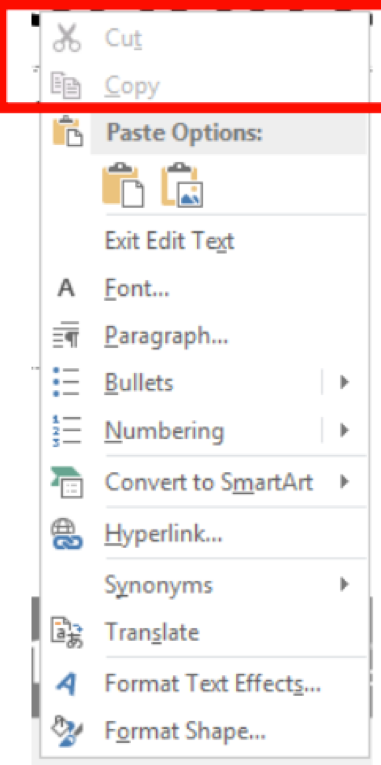
\includegraphics[width=0.3\linewidth]{constraint1}
\end{frame}

\begin{frame}
\frametitle{Constraints}
\centering
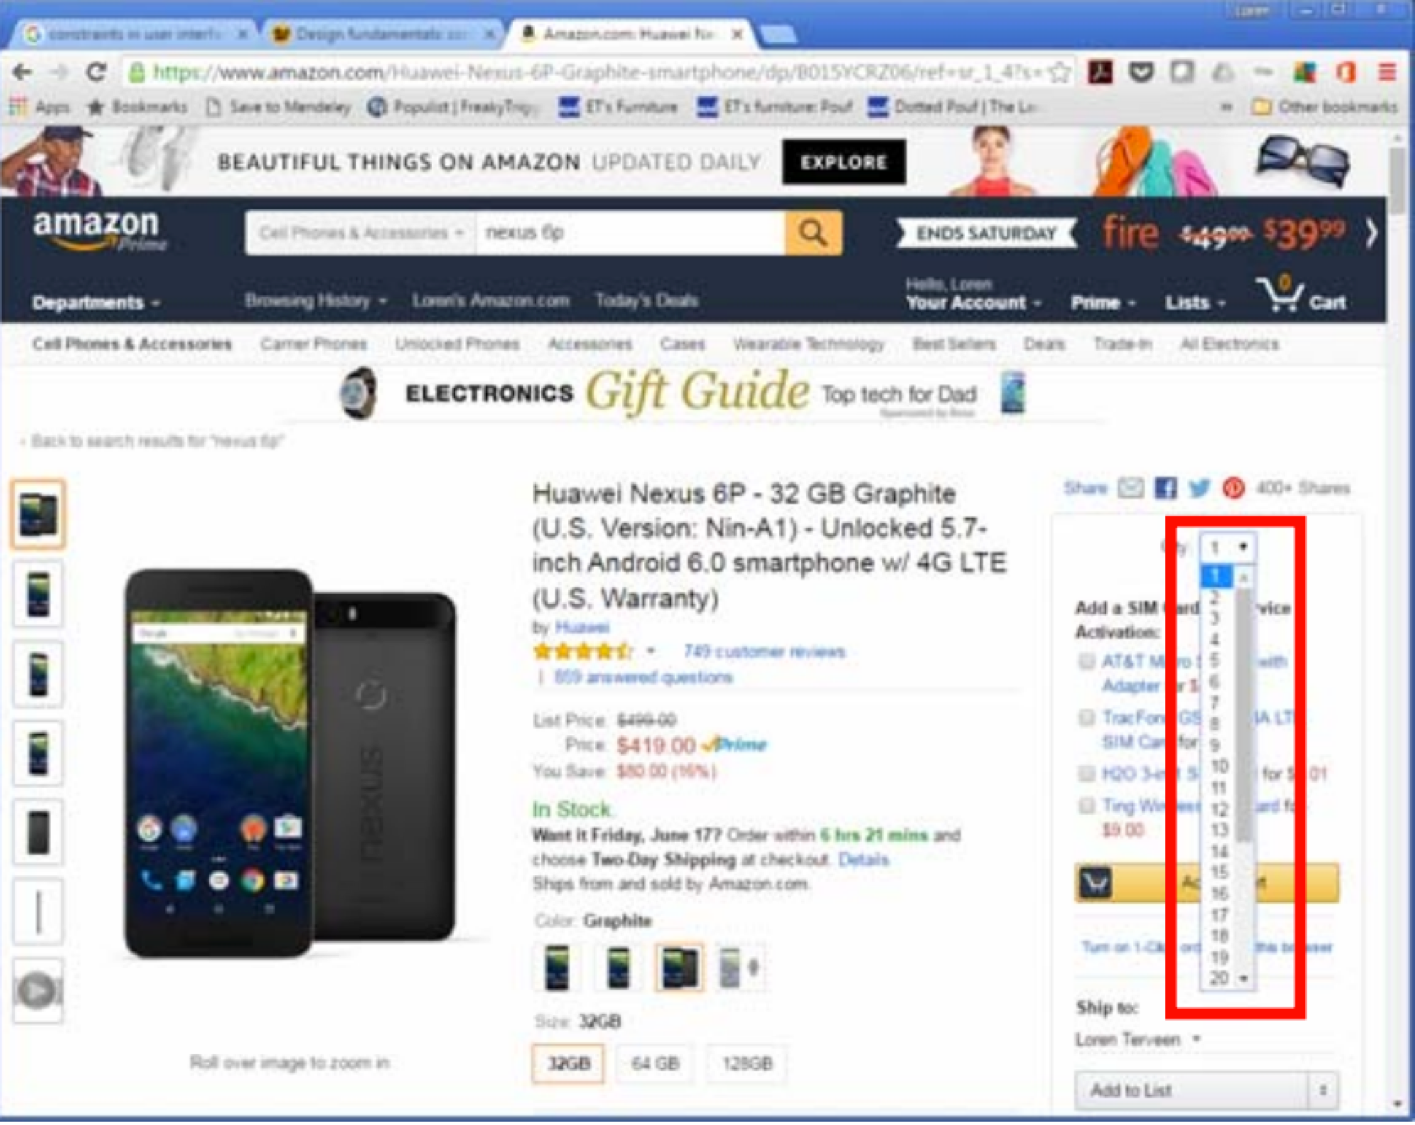
\includegraphics[width=0.7\linewidth]{constraint2}
\end{frame}

\begin{frame}
\frametitle{Constraints}
\centering
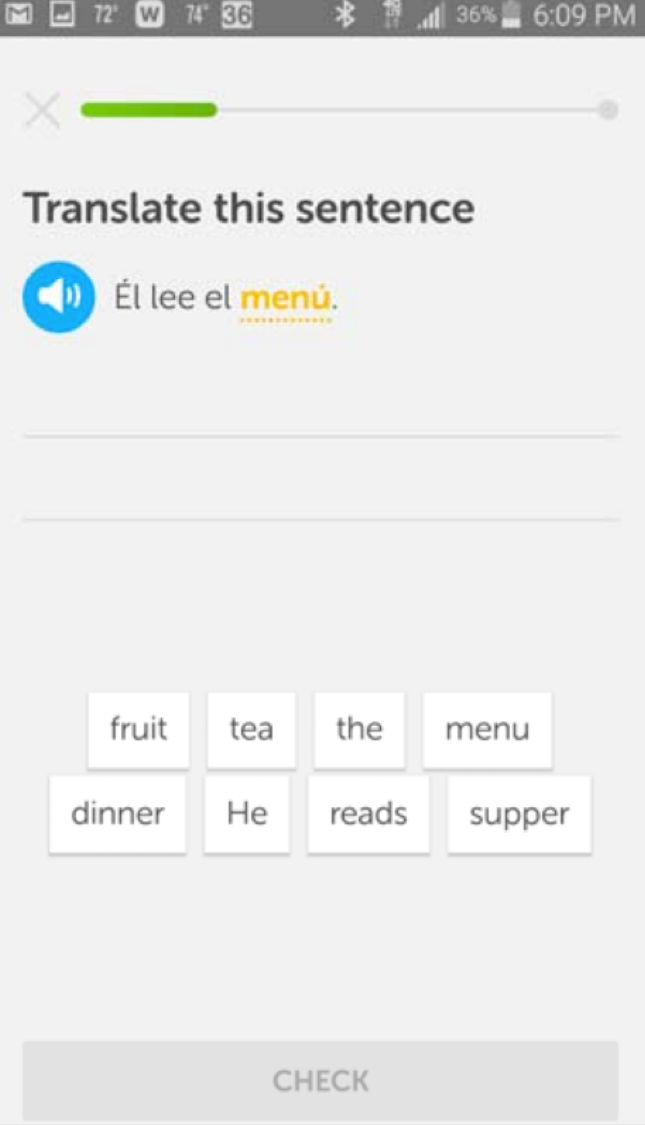
\includegraphics[width=0.3\linewidth]{constraint3}
\end{frame}

\begin{frame}
\frametitle{Constraints}
\centering
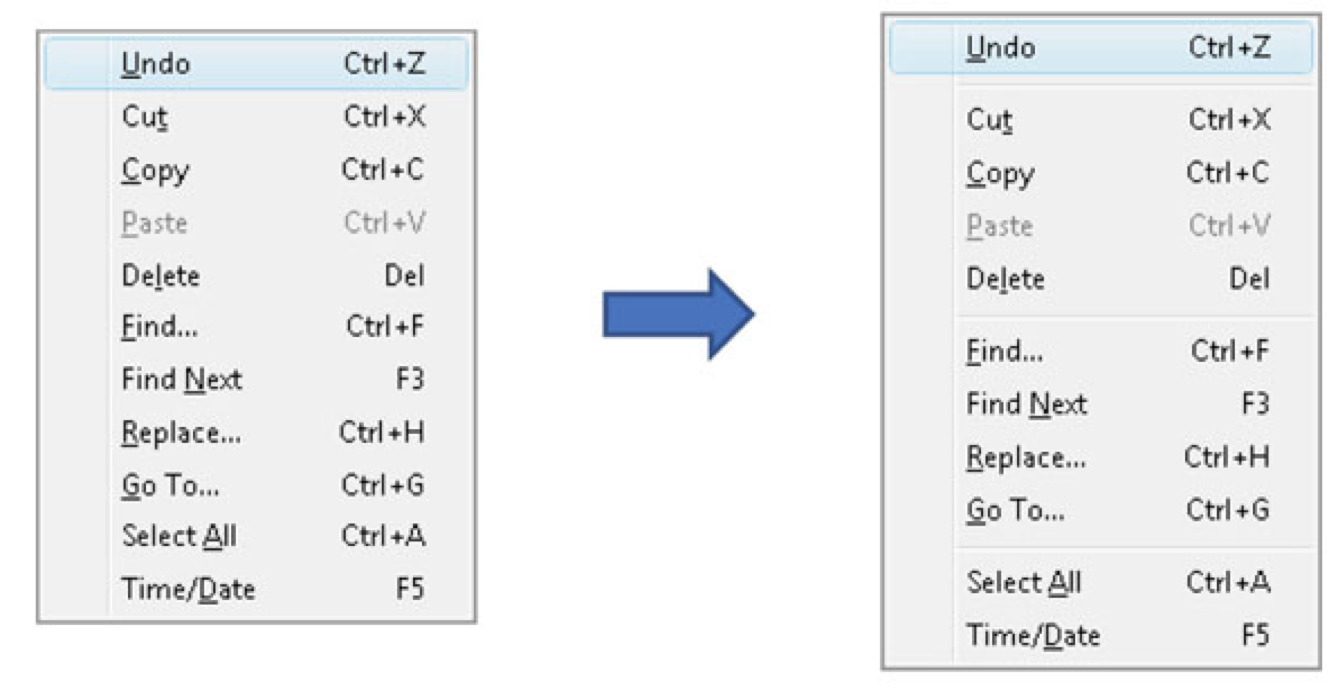
\includegraphics[width=0.7\linewidth]{constraint4}
\end{frame}

%
%\begin{frame}
%\frametitle{Constraints}
%\centering
%\begin{figure}
%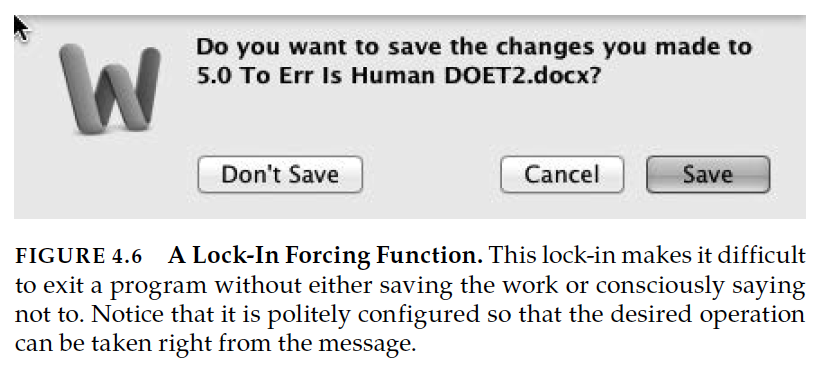
\includegraphics[width=0.6\linewidth]{force}
%\caption{Source: Fg 4.6 (Norman)}
%\end{figure}
%\end{frame}

\begin{frame}
\frametitle{Constraints}
\begin{columns}[c] % The "c" option specifies centered vertical alignment while the "t" option is used for top vertical alignment
	
	\column{.55\textwidth} % Left column and width
	\centering
	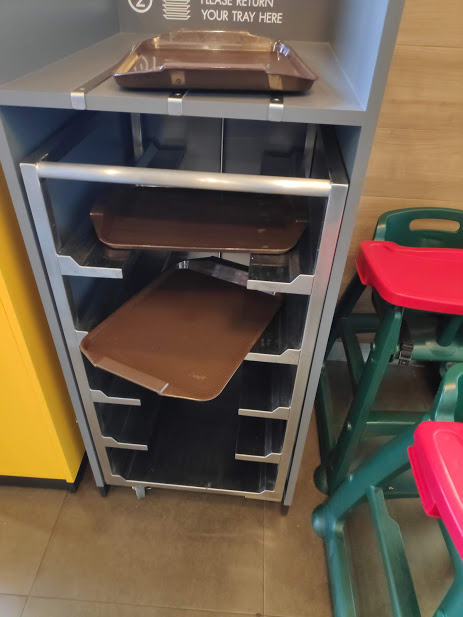
\includegraphics[width=0.7\linewidth]{mc}
	
	\column{.45\textwidth} % Right column and width
	\begin{itemize}
		\item How to better design this Mcdonald tray using the constraint concept?
	\end{itemize}
\end{columns}
\end{frame}

%\begin{frame}
%	\frametitle{Activities}
%	\begin{block}{Classwork}
%		Isn't it familiar where people forgets to take their card after using the ATM?  Attempt to redesign ATM to address this problem.\\
%		Submit your work to Google Classroom on HW4.
%	\end{block}
%	
%\end{frame}

\begin{frame}
\frametitle{Conventions}
Conventions are cultural constraints.  They are initially arbitrary, but evolve and become accepted over time.   They can vary enormously between cultures. \vfill

\centering
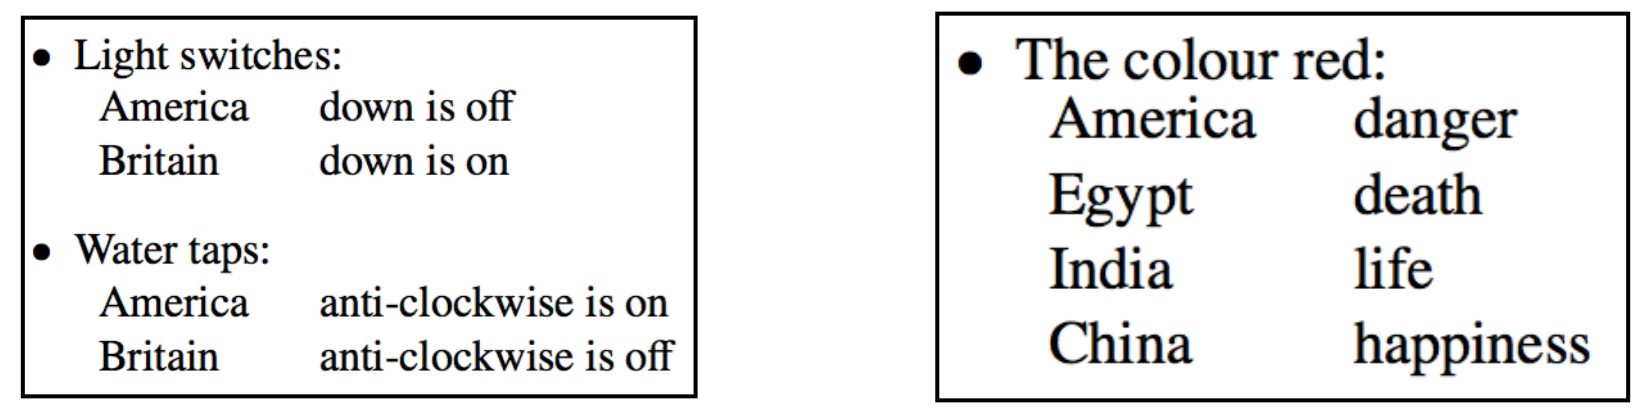
\includegraphics[width=0.9\linewidth]{convention}
\end{frame}

\begin{frame}
\frametitle{Conventions}
\begin{itemize}
	\item Avoid breaking conventions as it will add \textbf{confusion}
	\item For \textbf{website}, there are many conventions - where do you usually place logos in website?  Usually what is color of a link in website?  Where is the contact menu?  %Where is the search bar?  Where are the social media icons?  When you choose a range of price, what is the usual input style - a slider or a textbox? 
%	\item Violate conventions and people will complain.  Imagine US, they still yet to switch to metric system even though metric system is more precise!  You can always introduce \textbf{new} convention but do it only if they introduce \textbf{value} to customers.
	\item Never introduce your own psychology! 
	\item Designers have temptation to \textbf{reinvent} the wheel, because they \textbf{feel} they are hired to do something \textbf{new} and \textbf{different}
	\item It IS OK to introduce something new, but it should be with "really really good" reason, and always expect some complaints initially....
\end{itemize}
\end{frame}

\subsection{Consistency}

\begin{frame}
\frametitle{Consistency}
\begin{itemize}
	\item \textbf{Consistency} in design is virtuous.  When things are consistent, it becomes easy for users to catch the pattern, and thus learn. 
	\item Example: Ctrl-S, Cltr-C, Cltr-V   (This function is same across all applications)
\end{itemize}
\end{frame}

\begin{frame}
\frametitle{Consistency}
\centering
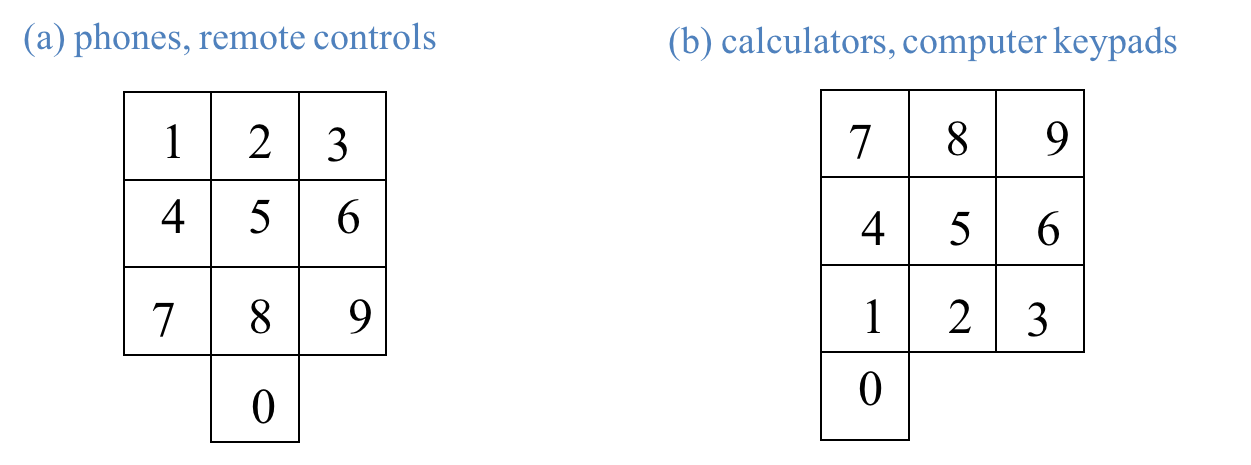
\includegraphics[width=1\linewidth]{consistent1}
\end{frame}


\begin{frame}
\frametitle{Consistency}
\centering
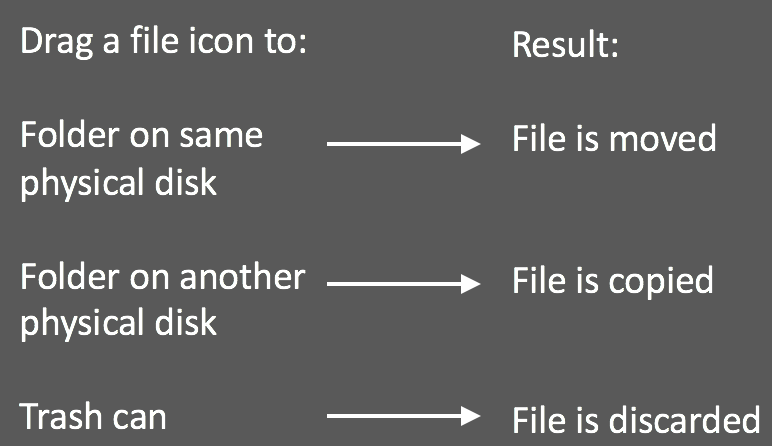
\includegraphics[width=0.9\linewidth]{consistent6}
\end{frame}

\begin{frame}
\frametitle{Consistency}
Important to allow users to observe any permanent states
\vspace{10pt}


\includegraphics[width=1\linewidth]{visible3}
\end{frame}

\begin{frame}
\frametitle{External consistency}
External consistency concerns the consistency with other elements in the same environment (e.g., Mac OS)
\vspace{10pt}


\includegraphics[width=0.8\linewidth]{consistent3}
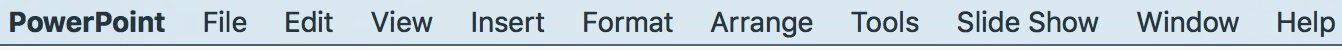
\includegraphics[width=0.8\linewidth]{consistent4}
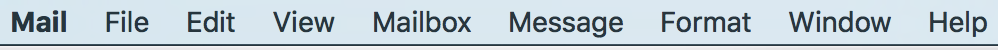
\includegraphics[width=0.7\linewidth]{consistent5}
\end{frame}

\begin{frame}
	\frametitle{Activities}
	\begin{block}{Classwork}
	\centering
	
\includegraphics[width=.5\linewidth]{elevator_bt}
	\begin{itemize}
		\item Attempt to redesign the elevator buttons so to \textit{minimize} people accidentally closing the door.
		\item Submit a screenshot and roughly 300 words arguing why you think your design will solve the problem to Google Classroom. 
	\end{itemize}
%		Put these design considerations in your design:\\
%1. People "loves" familiar design\\
%2. Not all people know English.  Reading also takes time!\\
%3. What color should be the button of Open and Close?  Does color even matters?
	\end{block}
\end{frame}

\begin{frame}
	\frametitle{Discussion}
\end{frame}


\begin{frame}
\Huge{\centerline{Questions}}
\end{frame}

%\begin{frame}
%	\frametitle{Reminders}
%	\begin{itemize}
%		\item \textbf{Project} - First paper reading summary due soon.  Hard copies on my shelf at the secretary room.  Soft copy on the Google classroom.
%	\end{itemize}
%\end{frame}

%\begin{frame}
%	\frametitle{Recap}
%	\begin{itemize}
%		\item Problems in design is \textbf{common}
%		\item Design is \textbf{difficult} due to its high \textbf{dimensionality}
%		\begin{itemize}
%			\item Tradeoffs
%			\item Context - use,  expertise, background, cultures,  user groups
%			\item User nature
%			\item Engineer nature
%		\end{itemize}
%		\item Remedies (often overlooked)
%		\begin{itemize}
%			\item Understand people \textbf{expectations} and background
%			\item Don't assume people will read or care
%			\item Remember \textbf{diversity}
%			\item Rapid \textbf{prototyping}
%			\item \textbf{Interview} but NOT follow
%			\item Understanding \textbf{goals}, not minimal/simpler/lookin' good
%			\item User \textbf{evaluation}
%			\item Design \textbf{principles} - Affordances, Constraints, Consistency
%		\end{itemize}
%	\end{itemize}
%\end{frame}

%\begin{frame}
%	\frametitle{CW1 Review}
%	\begin{itemize}
%			\item Discuss possible \textbf{tradeoffs}
%			\item \textbf{Convention} and familiarity
%			\item \textbf{Diversity}
%			\item Explain "\textbf{what}" cause the problem and "\textbf{why}" your solution works
%			\item Adding "\textbf{techie}" stuffs cautiously
%			\item Affordances, Constraints, Consistency, Mappings, Feedback
%			\item Needs user \textbf{evaluation} afterward
%		\end{itemize}
%\end{frame}

\subsection{Mapping}

\begin{frame}
\frametitle{Mapping}
\begin{itemize}
	\item \textbf{Mapping} is the spatial relationship between objects
	\item When the mapping uses\textbf{ spatial correspondence }, it is easy to determine how to use them.
	\item Mappings vary with \textbf{culture} - Arabic (right to left), Chinese (top to bottom), Roman (left to right).  So how to design an elevator buttons layout depends on \textbf{culture}
%	\item If you create an \textbf{universal} design, it is possible to break cultural convention, but expect a period of confusion before people adapt to them.  Also make sure people can \textbf{learn your system}
\end{itemize}
\end{frame}


\begin{frame}
\frametitle{Mapping}
\centering
\begin{figure}
	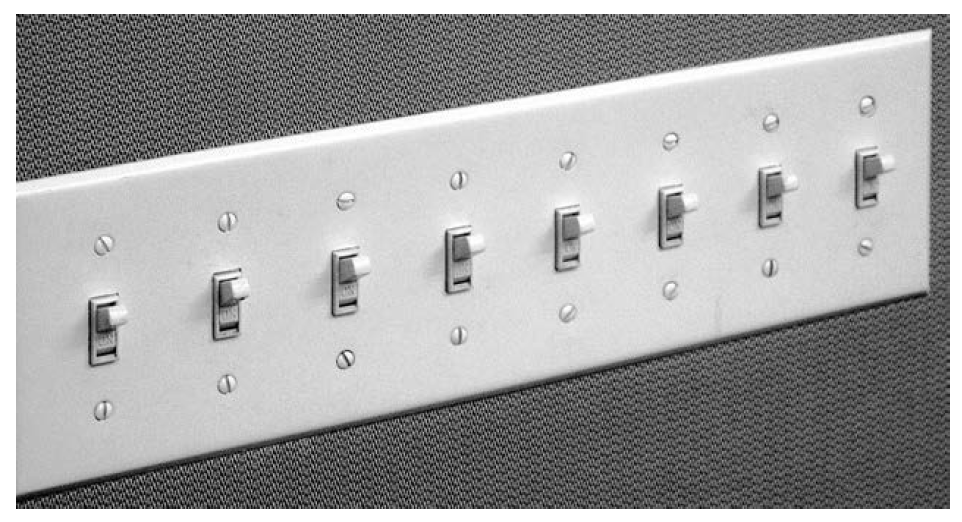
\includegraphics[width=0.8\linewidth]{badswitches}
	\caption{Source: Fg 4.4 (Norman) - Incomprehensible Light Switches}
\end{figure}
\end{frame}


\begin{frame}
\frametitle{Mapping}
\centering
\begin{figure}
	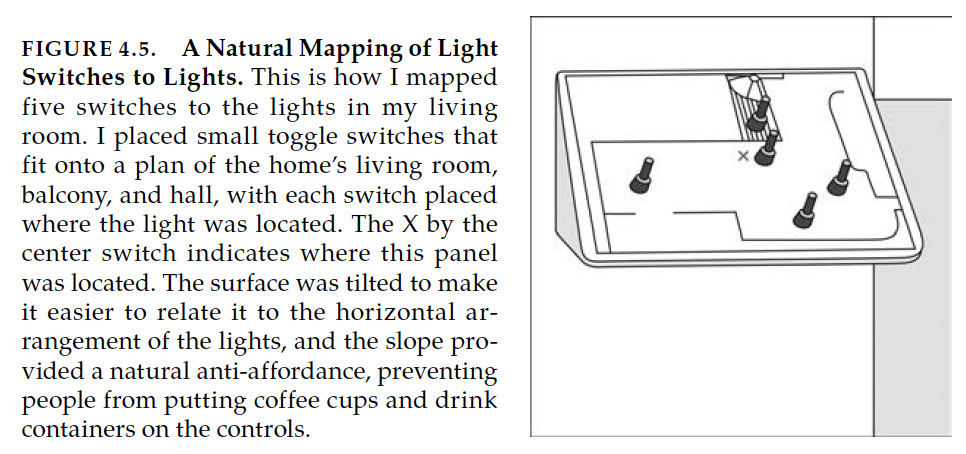
\includegraphics[width=1\linewidth]{goodswitches}
	\caption{Source: Fg 4.5 (Norman)}
\end{figure}
\end{frame}

\begin{frame}
\frametitle{Mapping}
\centering
\begin{figure}
	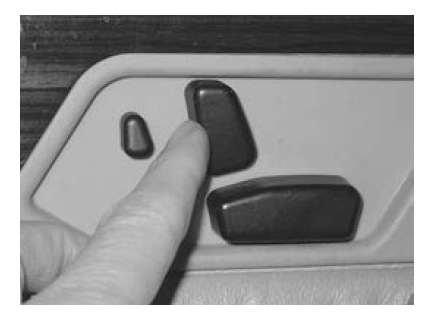
\includegraphics[width=0.6\linewidth]{map9}
	\caption{Source: Fg 1.7 (Norman)}
\end{figure}

\end{frame}

\begin{frame}
\frametitle{Mapping}
\centering
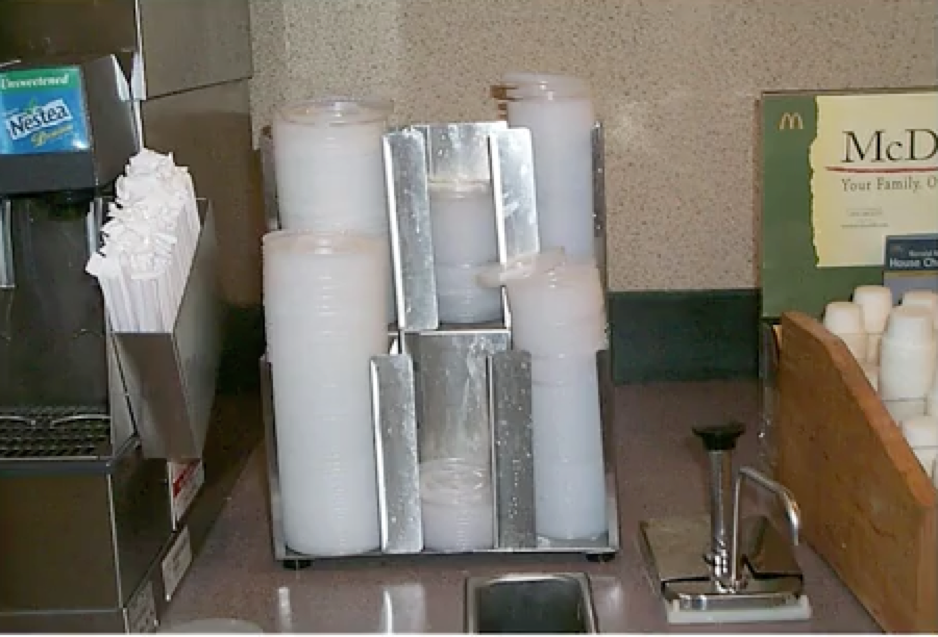
\includegraphics[width=0.8\linewidth]{map1}
\end{frame}

\begin{frame}
\frametitle{Mapping}
\centering
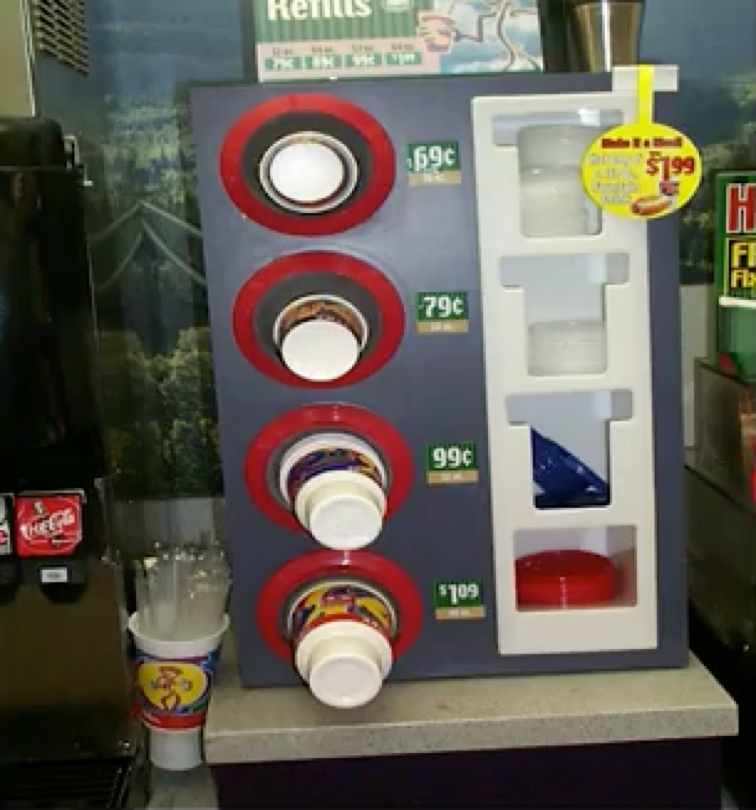
\includegraphics[width=0.5\linewidth]{map2}
\end{frame}

\begin{frame}
\frametitle{Mapping}
\centering
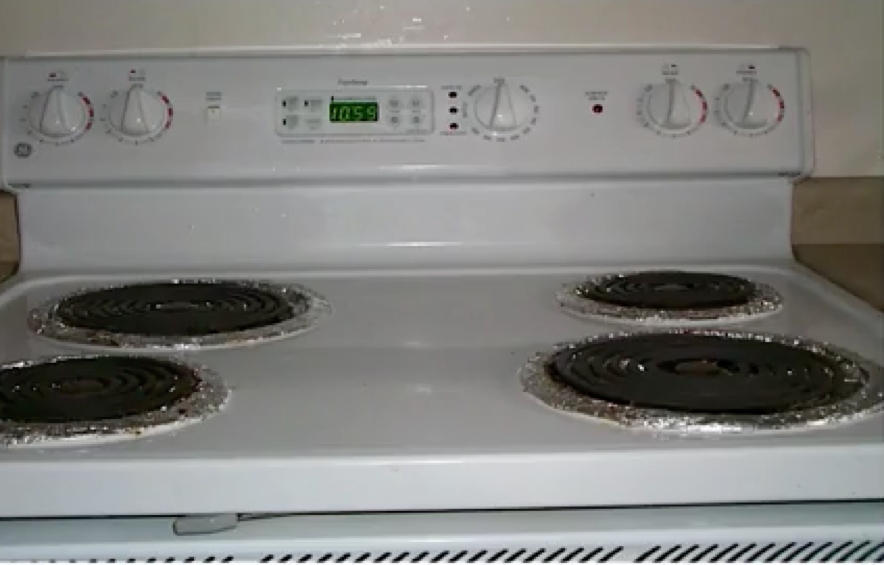
\includegraphics[width=0.9\linewidth]{map3}
\end{frame}

\begin{frame}
\frametitle{Mapping}
\centering
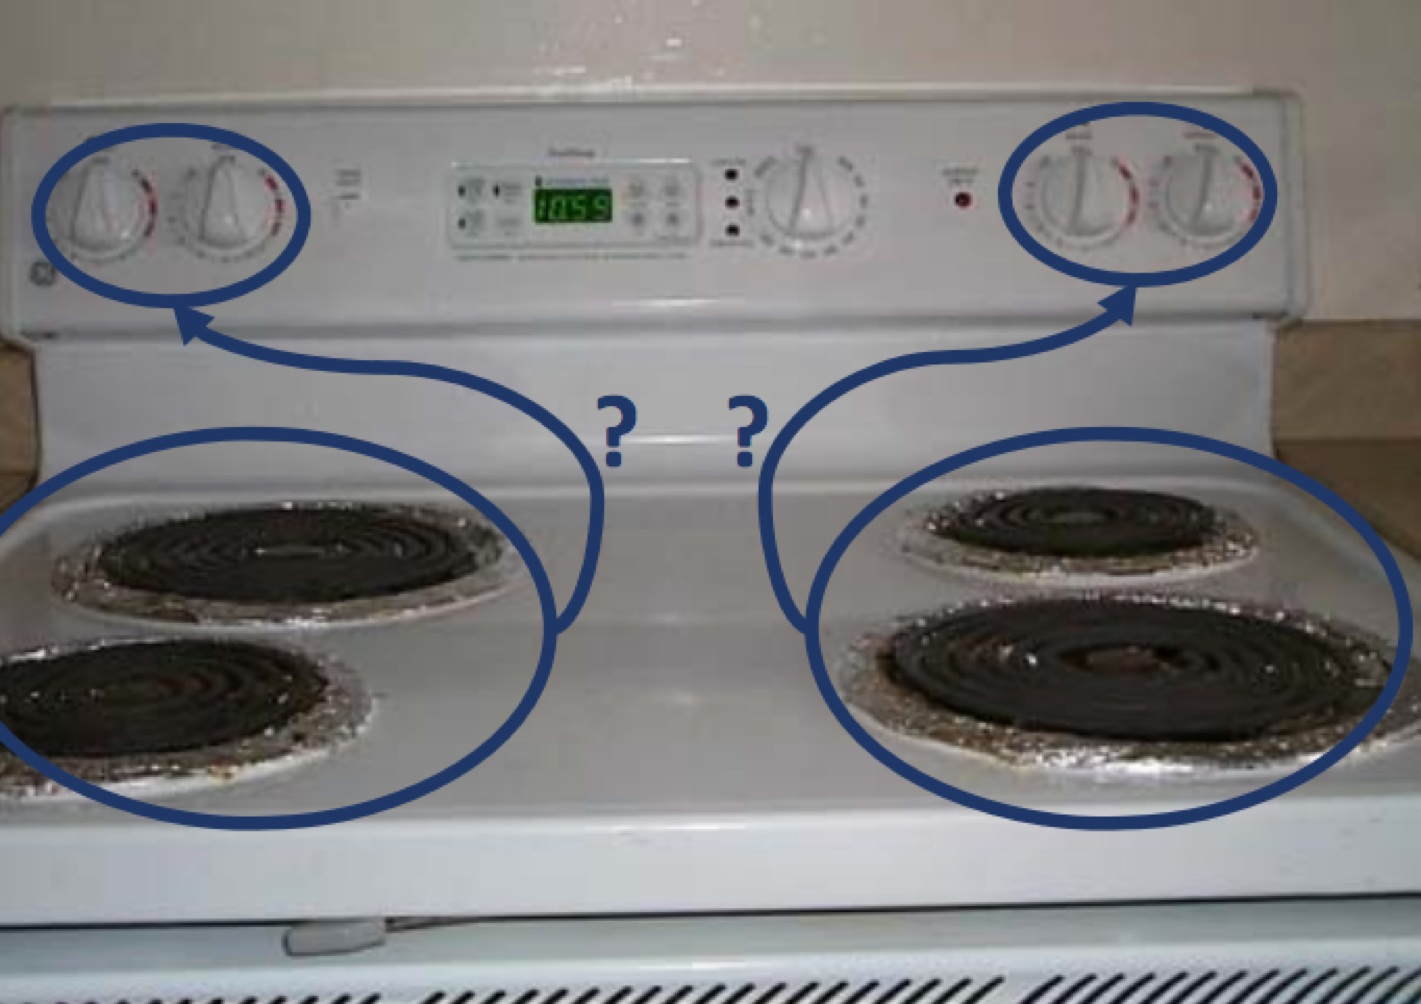
\includegraphics[width=0.8\linewidth]{map4}
\end{frame}

\begin{frame}
\frametitle{Mapping}
\centering
\includegraphics[width=0.8\linewidth]{map5}
\end{frame}

\begin{frame}
\frametitle{Mapping}
\centering
\includegraphics[width=0.9\linewidth]{map6}
\end{frame}

\begin{frame}
\frametitle{Mapping}
\centering
\includegraphics[width=0.9\linewidth]{map7}
\end{frame}

\begin{frame}
\frametitle{Mapping}
\centering
\includegraphics[width=0.4\linewidth]{map8}
\end{frame}

\begin{frame}
\frametitle{Mapping}
\centering
\includegraphics[width=0.3\linewidth]{elevator}
\end{frame}

\begin{frame}
\frametitle{Mapping}
\begin{columns}[c] % The "c" option specifies centered vertical alignment while the "t" option is used for top vertical alignment
	
	\column{.45\textwidth} % Left column and width
	\centering
	\includegraphics[width=1\linewidth]{switch}\newline
	
	\column{.55\textwidth} % Right column and width
	\begin{itemize}
		\item Oh my....there is a fire on my furnace....I got to turn it off...
		\item ....Oh no!  which one is off?
	\end{itemize}
\end{columns}
\end{frame}

\subsection{Feedback}
\begin{frame}
\frametitle{Feedback}
\begin{itemize}
	\item When there is \textbf{no feedback}, we get \textbf{confused}.  Why?
	\item Feedback must be \textbf{immediate} %even a delay of a tenth of a second can be devastating.   If the delay is too long, people often give up, and do other things.  
	\item Feedback must be \textbf{informative} - one flash and two flashes error message isn't very helpful
	\item \textbf{Too much feedback} can be annoying. Why? %Too much cause people to ignore them and turn them off
\end{itemize}
\end{frame}


\begin{frame}
\frametitle{Feedback}
\centering
\includegraphics[width=0.3\linewidth]{feedback1}
\end{frame}

\begin{frame}
\frametitle{Feedback}
\centering
\includegraphics[width=0.9\linewidth]{feedback3}
\end{frame}

\begin{frame}
\frametitle{Feedback}
\centering
\includegraphics[width=0.9\linewidth]{feedback4}
\end{frame}


\begin{frame}
\frametitle{Feedback}
\centering
\includegraphics[width=0.8\linewidth]{feedback}
\end{frame}


\begin{frame}
\frametitle{Feedback}

\begin{columns}[c] % The "c" option specifies centered vertical alignment while the "t" option is used for top vertical alignment
	
	\column{.35\textwidth} % Left column and width
	\includegraphics[width=1\linewidth]{instagram}
	
	\column{.65\textwidth} % Right column and width
	\begin{itemize}
		\item A clever trick Instagram uses to upload photo quick
		\item Whenever you upload a photo, Instagram will quickly finish uploading
		\item Trick users to think it finishes already
%		\item However, in fact, it is uploading in the background
%		\item Smart design that makes users feel "good"
	\end{itemize}
\end{columns}
\end{frame}


\begin{frame}
\frametitle{Feedback}

\begin{columns}[c] % The "c" option specifies centered vertical alignment while the "t" option is used for top vertical alignment
	
	\column{.35\textwidth} % Left column and width
	\includegraphics[width=1\linewidth]{youtube}
	
	\column{.65\textwidth} % Right column and width
	\begin{itemize}
		\item Human attention span is 8 secs (goldfish has a 12 secs!)
		\item 0.1 sec - is the limit that humans can wait while \textbf{manipulating}
		\begin{itemize}
			\item Important for direct manipulation, virtual world navigation
		\end{itemize}
		\item 1 sec - the limit that user's \textbf{flow of thoughts} go uninterrupted
		\begin{itemize}
			\item Display a busy cursor if things take longer than 1 sec
		\end{itemize}
		\item 10 sec - the limit that user can \textbf{wait}
		\begin{itemize}
			\item Display a progress bar if things take longer than 10 sec
		\end{itemize}
	\end{itemize}
\end{columns}
\end{frame}

%
%\begin{frame}
%	\frametitle{Activities}
%	\begin{block}{Classwork}
%		Miss Universe 2015 was an embarrassing moment where winners were announced wrong.  First, discuss why such errors happen in the first place.  Then attempt to redesign.
%		\centering
%		\includegraphics[width=.6\linewidth]{universe}
%		\\
%		Submit this work to Google Classroom on HW6.
%	\end{block}
%	
%\end{frame}

%\begin{frame}
%\begin{center} 
%\usebeamerfont*{frametitle} \usebeamercolor[fg]{frametitle}  5-mins break 
%\end{center}
%\end{frame}

\section{Design Theory}

\subsection{Mental Models}
\begin{frame}
\frametitle{So...what's a successful design?  - Mental Models}
\begin{itemize}
%	\item Matches of mental models is a characteristics of a successful design
	\item \textbf{Mental model} is how one thinks something works
	\item \textbf{If designer and user mental model matches, it is a successful design}
	\item \textbf{Good} mental model examples: 
	\begin{itemize}
		\item Folder and files icons
		\item Scissors
	\end{itemize}		
	\item Matching mental model is \textbf{hard}.  Novice and experts, for example, have completely different models.   Designers and users also have often very different models
%	\item Mental models comes from \textbf{device itself}, comes from \textbf{reading}, but usually from \textbf{experience}.    
\end{itemize}
\end{frame}


\begin{frame}
\frametitle{Mental Models}
\centering
\begin{figure}
	\includegraphics[width=0.6\linewidth]{model}
	\caption{Source: Fg 1.8 (Norman)}
\end{figure}
\vspace{-10pt}
\begin{itemize}
	\item When users have incorrect mental models, your design fails
	\item \textbf{Watch}: There are five buttons.  There are \textbf{affordances} of buttons but it does not \textbf{signifies} what to do.  There are also no clear \textbf{mappings} between functions and buttons.   \textbf{Constraints} are also not applied properly - each button can be pressed or hold or press twice, none of which are explained clearly.   Only way to use this watch is to read the manual....too bad
\end{itemize}
\end{frame}


\begin{frame}
\frametitle{Mental Models}
\centering
\begin{figure}
	\includegraphics[width=0.6\linewidth]{model2}
	\caption{Source: Fg 1.9 (Norman)}
\end{figure}
\vspace{-10pt}
\begin{itemize}
	\item \textbf{Refrigerator}: If the freezer is too cold, what you will do?
\end{itemize}
\end{frame}

\begin{frame}
\frametitle{Mental Models}
\centering
\begin{figure}
	\includegraphics[width=0.7\linewidth]{model3}
	\caption{Source: Fg 1.10 (Norman)}
\end{figure}
\end{frame}

%\begin{frame}
%\frametitle{Mental Models}
%\centering
%\begin{figure}
%	\includegraphics[width=1\linewidth]{model4}
%	\caption{Source: Fg 1.11 (Norman)}
%\end{figure}
%\end{frame}

%\begin{frame}
%\frametitle{Paradox of Technologies and Design Challenges}
%\begin{itemize}
%	\item It is no doubt technologies \textbf{simplify} our life.    Yet, the more functions \textbf{complicate our life} by making the system harder to learn, harder to use.  This is designers' challenge
%	\item Desgin requires the cooperative efforts of multiple disciplines, but another paradox is that \textbf{each discipline believe their contribution to be most important} - \textbf{Price} says the marketing, \textbf{reliability} says the engineers, \textbf{user experience} says the designers, but in fact, successful products satisfy all requirements.  This is another big challenge - the collaboration between disciplines
%\end{itemize}
%\end{frame}

\subsection{Don't Make Me Think}

\begin{frame}
	\frametitle{Don't Make Me Think}
	\begin{itemize}
		\item Famous book of Steve Krug's \textit{Don't Make Me Think}
		\item Key concept of the book is \textbf{Don't make users think}
		\item \textbf{Not thinking} means that users should be able to quickly reach their goal without unnecessary cognitive effort
%		\item On the other hand, \textbf{thinking} means that users struggle with many usability problems and have to \textbf{think} to overcome those problems
%		\item The point is, when we’re using the Web every question mark adds to our  \textbf{cognitive workload}, \textbf{distracting our attention} from the task at hand. The distractions may be slight but they add up
	\end{itemize}
\end{frame}

\begin{frame}
	\frametitle{Don't Make Me Think}
	\centering
	\begin{figure}
		\includegraphics[width=0.7\linewidth]{steve/not-thinking}
		\caption{Source: Pg. 12 (Steve)}
	\end{figure}
\end{frame}

\begin{frame}
	\frametitle{Don't Make Me Think}
	\centering
	\begin{figure}
		\includegraphics[width=0.8\linewidth]{steve/thinking}
		\caption{Source: Pg. 13 (Steve)}
	\end{figure}
\end{frame}

\begin{frame}
	\frametitle{Things that Make Us Think - Names}
	\begin{itemize}
		\item Typical culprits include cute or clever \textbf{names}, marketing-induced names, company-specific names, and unfamiliar names
	\end{itemize}
	\centering
	\begin{figure}
		\includegraphics[width=0.8\linewidth]{steve/names}
		\caption{Source: Pg. 14 (Steve)}
	\end{figure}
\end{frame}

\begin{frame}
	\frametitle{Things that Make Us Think - Links and Buttons}
	\begin{itemize}
		\item Needless source of question marks over people's heads is \textbf{links and buttons that aren't obviously clickable}.  The point is simple things like links should not cause any such headache
	\end{itemize}
	\centering
	\begin{figure}
		\includegraphics[width=0.8\linewidth]{steve/links}
		\caption{Source: Pg. 15 (Steve)}
	\end{figure}
\end{frame}

\begin{frame}
	\frametitle{Things that Make Us Think - Search}
	\begin{itemize}
		\item Many bookstore sites require us to \textbf{think how we want to search} which adds up the cognitive effort 
	\end{itemize}
	\centering
	\begin{figure}
		\includegraphics[width=0.5\linewidth]{steve/search}
		\caption{Source: Pg. 16 (Steve)}
	\end{figure}
\end{frame}

\begin{frame}
	\frametitle{How We Really Use the Web}
	\begin{itemize}
		\item A gap often between how we think people use Websites and how they actually use them
		\item In fact, people mostly is \textbf{impatient} and usually in hurry, only care about their \textbf{goal}, \textbf{does not like to think}
		\item Thus, most people will just \textbf{scan} and \textbf{click}, within tenth of a second...
	\end{itemize}
		\begin{figure}
		\includegraphics[width=0.5\linewidth]{steve/how}
		\caption{Source: Pg. 21 (Steve)}
	\end{figure}
\end{frame}

\begin{frame}
	\frametitle{Fact of Life I - We scan}
	\begin{itemize}
		\item We don't read.  We scan.  We are smart to know we do not need to read everything
	\end{itemize}
	\begin{figure}
		\includegraphics[width=0.7\linewidth]{steve/fact1}
		\caption{Source: Pg. 23 (Steve)}
	\end{figure}
\end{frame}

\begin{frame}
	\frametitle{Fact of Life II - local optima}
	\begin{itemize}
		\item We don't choose the \textbf{best} option.  We choose the \textbf{first reasonable} option because
		\begin{itemize}
			\item We are usually in a \textbf{hurry}
			\item The \textbf{penalty} for guessing wrong is low with the Back button always available
			\item Not to mention guessing is \textbf{fun} 
		\end{itemize} 
	\end{itemize}
\end{frame}

\begin{frame}
	\frametitle{Fact of Life III - We don't like to learn/think}
	\begin{itemize}
		\item We don't like to think or learn, we usually just \textbf{muddle through} 
%		\item Why is that?  Because it's not important to us whether we understand everything.  
%		\item Almost all (if not all) users (including smart people) don't like to learn or think.   
		\item If we find something that works, we stick to it, we \textbf{hardly change our way}
%		\item Designers are usually surprised of user behaviors, because they \textbf{thought everyone are just like them} who are interested in how things work
	\end{itemize}
\end{frame}

%\subsection{Three Levels of Processing}
%
%\begin{frame}
%\frametitle{Three Levels of Processing}
%Three levels of emotional-cognitive processing:
%	\begin{enumerate}
%		\item \textbf{Visceral} - the quick, automatic, and subconscious judgments; the first impression; the immediate perception; minimal learning involve. Linked with motor systems (fight or flee).  Design aesthetics drive these responses.
%		\item \textbf{Behavioral} - relates to experience when performing actions and every action is associated with an expectation  Most action in this level is subconscious.  %A state \textbf{flow} happens when challenge of activity just slightly exceeds our skill.%
%		\item \textbf{Reflective} - relates to home of conscious cognition.  This is your experience after conscious reasoning.  Highest levels of emotions comes from this level.    %Emotion and cognition are tightly intertwined 
%	\end{enumerate}
%\end{frame}
%
%\begin{frame}
%\frametitle{Three Levels of Processing}
%\begin{itemize}
%	\item Good design satisfy all levels
%	\item But for designer, \textbf{reflection} is perhaps the most important because it is conscious and emotions are highest
%	\item \textbf{Reflection as the decider} - if you have strong positive visceral experience but some usability problems at the behavioral level, your reflections may overlook these usability problems..  On the other hand, if you have too many usability problems, your reflections may overlook the strong positive visceral experience
%%	\item At the end, the \textbf{philosophy} or what \textbf{high-level value} you provide to your customer is most important.  Company that\textbf{ understand their why} is most successful
%\end{itemize}
%\end{frame}


%\begin{frame}
%\frametitle{Three Levels of Processing}
%\begin{itemize}
%	\item In psychology, long debase whether emotion or cognition happens first
%	\item Both because \textbf{they affect/trigger one another. } You feel hungry, thus you find food.  You are thinking about food, thus you feel hungry.
%	\item Thus, all three levels of processing determine a person's cognitive and emotional state.
%\end{itemize}
%\end{frame}

%\begin{frame}
%	\frametitle{Self-Evident Design}
%	\begin{itemize}
%%		\item Because most people are in such a hurry, design all be self-evident and obvious.  Not to mention that winners between two designs are due to only very minor details. \textbf{Self-Evident Design} may be achieved with:
%		\item Clear \textbf{visual hierarchy} i.e., use mapping
%		\item Take advantage of \textbf{conventions}
%		\item  Don't argue but \textbf{test}
%		\item Design for both novice and expert users - allow multiple endings
%		\begin{itemize}
%		\end{itemize}
%	\end{itemize}
%\end{frame}
%
%
%\begin{frame}
%\frametitle{Design for Boundary Users, Not Average}
%\begin{itemize}
%	\item The experience level of people using computer software tends, like most population distributions, to follow the classical statistical \textbf{bell curve }(normal distribution).
%	\item Beginners do not remain beginners for long
%	\item The difficulty of maintaining a high level of expertise means that experts fade over time
%	\item \textbf{Most users gravitate over time towards intermediacy}
%	\item \textbf{Do not design for the average user}; it produces a design to please no-one
%\end{itemize}
%\centering
%\includegraphics[width=0.6\linewidth]{user2/3}
%\end{frame}
%
%\begin{frame}
%\frametitle{Design for Boundary Users, Not Average}
%\begin{itemize}
%\item Users form a point cloud
%\end{itemize}
%\centering
%\includegraphics[width=0.7\linewidth]{user/10}
%\end{frame}
%
%\begin{frame}
%\frametitle{Design for Boundary Users, Not Average}
%\begin{itemize}
%\item Average users
%\end{itemize}
%\centering
%\includegraphics[width=0.7\linewidth]{user/11}
%\end{frame}
%
%\begin{frame}
%\frametitle{Design for Boundary Users, Not Average}
%\begin{itemize}
%\item If our design \textbf{satisfies the hard cases around the edges}, the ones in the middle should be able to use the interface as well.
%\end{itemize}
%\centering
%\includegraphics[width=0.7\linewidth]{user/12}
%\end{frame}

%\begin{frame}
%	\frametitle{Activities}
%	\begin{block}{Classwork}
%		\footnotesize
%		Go to the internet, and capture 5 screenshots of random parts of a website which you think violates "Don't make me think".  (1) Explain why you think it's bad, and (2) Attempt to redesign the drawings.
%		\centering
%		\includegraphics[width=.4\linewidth]{sis}\\
%		Submit your work on Google Classroom on HW7.
%	\end{block}
%	
%\end{frame}

%\begin{frame}
%	\frametitle{Activities}
%	\footnotesize
%	\begin{block}{Classwork}
%		Isn't it familiar where people forgets to take their card after using the ATM?  Attempt to redesign ATM to address this problem.\\
%		\vspace{0.3cm}		
%		Put these design considerations:\\
%		1.  If you use blinking, how strong or subtle should it be.  What color should you use?  What if the user is blind?\\
%2.  If you use blinking in some other places, maybe user is looking at the screen and did not see the blinking, or maybe user is looking at the money slot where the money is coming out....\\
%3.  If you use sound, maybe it is too loud!  What if the user is deaf?\\
%4.  If you put text on the screen after withdrawing, maybe some people instead focus on the logo of the bank and ignore the text!		\\
%	\end{block}
	
%\end{frame}



%\begin{frame}
%	\frametitle{Reminders}
%	\begin{itemize}
%		\item \textbf{HW7} due today
%		\item \textbf{HW8} due next Monday
%		\item \textbf{Project leaders} - Second paper reading summary due next Monday and writing the first proposal on the following week.   Don't forget the \textbf{hard copy }on class next Monday for the summary.
%	\end{itemize}
%\end{frame}

%\begin{frame}
%\frametitle{Assignment (Individual)}
%Access the homework via Google Classroom (code found at the intro slide)
%\begin{figure}
%	\includegraphics[width=1\linewidth]{assignment}
%\end{figure}
%\end{frame}

\begin{frame}
	\frametitle{Activities}
	\begin{block}{Classwork}
		\footnotesize
		Shower at hotel is something simple that is often frustrating.  Have your encounter relatives where they have difficulty understanding how the shower works?  Have you ever turn on the shower with water splash right on your face when it's not intended?  Attempt to redesign the shower system. \\
		\centering
		\includegraphics[width=.3\linewidth]{faucet}
	\end{block}
\end{frame}


\begin{frame}
	\frametitle{Discussion}
\end{frame}

%\begin{frame}
%	\frametitle{Activities}
%	\begin{block}{Classwork}
%		\footnotesize
%		Put these design considerations into your design:\\
%1. Don't assume hot is on the right and cold is on the left.   This depends on culture and it is dangerous to design in that way.  For example, UK people may think left is hot, while US people think that left is cold.  Avoid this mistake.\\
%2.  Take care of the affordances.  If you use a handle, this implies "continuous" scale.  If you use a button, it implies "binary" scale.  Be extremely careful.\\
%3. Where should the default temperature be?  How it should be set?  Should it be reset after use?\\
%4. How do you smartly switch mode between shower and faucet?  Which one should be default?  Should I be able to use both at the same time?\\
%5. How to best represent temperatures?  Should it be absolute (37.2 C) or should it be relative (cold, hot, hotter, hottest)?\\
%	\end{block}
%	
%\end{frame}

\begin{frame}
\frametitle{What's next}
Read my slide on \textbf{Writing},
	\begin{itemize}
		\item Learning how to actually write
		\item Perform some reading workshop together
	\end{itemize}
\end{frame}

\begin{frame}
\Huge{\centerline{Questions}}
\end{frame}

%\section{Appendix}
%
%\subsection{Shneiderman's Eight Golden Rules of Interface Design}
%\begin{frame}
%\frametitle{Shneiderman's Eight Golden Rules of Interface Design}
%\begin{enumerate}
%	\item Strives for \textbf{consistency}: consistent aesthetics, terminologies, layout ease learning process
%	\item Seek \textbf{universal usability}: Recognize the needs for diverse users - novice vs. experts, age ranges, disabilities, culture, expertise.  For example, add explanations for novices, but also add shortcuts for experts.  Allowing multiple ways of doing same thing.
%	\item Offer \textbf{informative feedback}: For frequent actions, response can be modest.  For infrequent and major actions, response should be substantial.  Avoid non-informative feedback.
%	\item Design \textbf{dialogs} to yield closure: Sequence of actions organizes into groups with a beginning, middle, and end, e.g., checkout process.  By leading users, it avoids confusion and errors.
%\end{enumerate}
%\end{frame}
%
%\begin{frame}
%\frametitle{Shneiderman's Eight Golden Rules of Interface Design}
%\begin{enumerate}
%\item Prevent \textbf{errors}: design so that users cannot make \textbf{serious} errors by graying out items, form validations, provide informative feedback
%\item Permit easy \textbf{reversal of actions}: actions should be reversible to relieve anxiety and encourages exploration
%\item Keep users in \textbf{control}: Experienced users want to be in control, get annoyed by tedious data-entry, get annoyed by new convention.  Enable control through customization and shortcuts
%\item Reduce \textbf{short-term memory} load: Human have limited short-term memory (rule of thumb is that people can remember seven plus or minus two chunks; for Steve Job, people can best remember three points); lengthy forms, action recall, for example, should be avoided
%\end{enumerate}
%\end{frame}
%
%\subsection{Design Thinking}
%
%\begin{frame}
%\frametitle{Design Thinking}
%\begin{columns}[c] % The "c" option specifies centered vertical alignment while the "t" option is used for top vertical alignment
%	
%	\column{.35\textwidth} % Left column and width
%	\begin{figure}
%		\includegraphics[width=0.8\linewidth]{process}
%		\caption{Source: Figure 6.2 (Norman)}
%	\end{figure}
%	
%	
%	\column{.65\textwidth} % Right column and width
%	
%\begin{itemize}
%	\item Design thinking is the process for \textbf{solving design problems}, focusing on iterative and empathy approach
%\end{itemize}
%	
%\end{columns}
%
%
%\end{frame}
%
%%\begin{frame}
%%\frametitle{Design Thinking}
%%\begin{itemize}
%%	\item \textbf{Observation} - This is the initial \textbf{trigger} for \textbf{problem identification}.  You  either experience personally,  listen to others' account of an existing problems, or observe people difficulties in performing task.   One of the most important task here is to \textbf{first understand your users.}
%%	\item \textbf{Idea Generation} - You will come up with numerous ideas (it is dangerous to come up with only one idea).  Also it is highly possible you need to read existing papers to understand what has been done and their limitations.  
%%	\item \textbf{Prototyping} - The only way to know whether an idea is working is to test it.  Build a quick prototype or mockup.  Mockups can be pencil sketches, foam and cardboard models, or simple images
%%\end{itemize}
%%\end{frame}
%%
%%\begin{frame}
%%\frametitle{Design Thinking}
%%\begin{itemize}
%%	\item \textbf{Testing/Evaluation} - Gather people who corresponds closely to your \textbf{target population }.  Set hypotheses.  Then, usually, formal approach is recommended, where both quantitative and qualitative responses are recorded.  Video recordings and interviews are effective to understand users' thoughts and actions.  6-20 participants are standard
%%	\item \textbf{Iteration} - One is impossible to get the design right at the first time.    Thus designers have to \textbf{fail frequently, and fail fast}
%%\end{itemize}
%%\end{frame}
%
%\begin{frame}
%\frametitle{(1) Observation - Classification}
%\centering
%%\includegraphics[width=0.5\linewidth]{user2/2}
%\begin{itemize}
%	\item The first step is to first \textbf{understand your users}.  
%	\item Classifications often help.  Users can be classified according to their:
%	\begin{itemize}
%		\item Educational level, Age, Gender, Assumptions
%		\item \textbf{Expertise}: experience of computers in general, understanding of the task domain%, and expertise in using the specific system.
%		\item \textbf{Goals}: Low-level and High-level
%	\end{itemize}
%\end{itemize}
%\end{frame}
%
%\begin{frame}
%\frametitle{(1) Observation - Interview}
%\begin{itemize}
%%	\item \textbf{One-on-one interviews} are often more effective to discover hidden problems
%%	\item Make sure you interview with \textbf{target population}
%	\item Designers need to be aware of:
%	\begin{itemize}
%			\item Most people \textbf{does not understand their own behavior}
%			\item Rather than ask, sometimes it is better to \textbf{observe} how user use the tools
%			\item \textbf{Do not always follow} your user, understand why and what they really need
%			\item \textbf{Clarifying questions} in the context of use
%	\end{itemize}
%	\item Key things to ask: (1) \textbf{current way of doing things},  (2) \textbf{current problems},  and (3) \textbf{what they truly want to achieve (goal) }
%%	\item You may ask users for solutions but be cautious.   What we want is to understand the problem, not solution. You may also be \textbf{mislead by users}
%\end{itemize}
%\end{frame}
%
%\begin{frame}
%\frametitle{Etiquette of Interview}
%\begin{itemize}
%	\item Avoid \textbf{biases}, focus on listening, don't talk too much...
%	\begin{itemize}
%		\item\textit{ Are you happy in the products} [encourage \textbf{bias}]?
%		\item \textit{But I think you may not be thinking right} [providing \textbf{unnecessary opinions}]?
%		\item \textit{Hmm....}[Showing \textbf{unnecessary approval}]...
%	\end{itemize}
%	\item Ask open-ended questions
%	\item Use closed-questions to clarify your answer
%	\item Keep on asking \textbf{why why why} to understand their goals and how they reach their goals
%	\item \textbf{Summarize} your points to interviewers
%\end{itemize}
%\end{frame}
%
%%\begin{frame}
%%\frametitle{Tasks are not Goals}
%%\begin{itemize}
%%\item Goal: Get something to eat.
%%\item Task: Go to the restaurant around the corner
%%\item Task: Call the pizza delivery service, Or
%%\item Task: Go to the supermarket, buy ingredients, and cook for myself
%%\end{itemize}
%%Too often, designers focus on simplifying a task, rather than accomplishing a goal.  Tasks are a means to an end, not an end in themselves.
%%\end{frame}
%
%\begin{frame}
%\frametitle{(2) Ideation}
%\begin{itemize}
%	\item Rules for brainstorming
%	\begin{enumerate}
%		\item No one is allowed to \textbf{criticize} another’s ideas. 
%		\item Programmers must \textbf{not say no}  %it cannot be implemented. 
%		\item Graphic designers must not \textbf{laugh} %at programmers’ drawings.
%		\item Propose \textbf{multiple alternatives}
%		\item Be as \textbf{crazy} and \textbf{foolish} as possible (but serious)
%		\item \textbf{Respect}
%	\end{enumerate}
%	\item Only \textit{after}, organize ideas and rank them according to:
%	\begin{itemize}
%		\item \textbf{Novelty} - what is new here? Did you carefully check that no one has done this before?
%		\item \textbf{Feasibility} - given time, skill, resource, can you really achieve?
%		\item \textbf{Effective} - does your system truly solve the existing root-cause problem?
%	\end{itemize}
%\end{itemize}
%\end{frame}
%
%\begin{frame}
%	\frametitle{(2) Ideation}
%	\begin{itemize}
%		\item\textbf{Getting ideas from others} are helpful such as reading papers, observing people, or talking with other designers 
%%		\item Some designers are afraid to be influenced by others' ideas.  What's wrong with this thought?
%		\item Two top-tier conferences in HCI includes \textbf{CHI} and \textbf{UIST} 
%		\item \textbf{Trick}: Start with only 1 key paper you really like. Perform \textbf{snowballing} (the paper references) and \textbf{backtracking} (who cites the paper) %to understand the web of related works.   May be daunting task to find 20+ papers related to your topic.  The trick is to 
%	\end{itemize}
%\end{frame}
%
%\begin{frame}
%\frametitle{(3) Prototyping}
%\centering
%"There's a mantra at IDEO: "\textbf{Never go to a meeting without a prototype}."  At whatever stage of development, one week, one month, or 6 months."
%\newline
%- Tim Brown, President, IDEO, CHI 2004
%\end{frame}
%
%%
%%\begin{frame}
%%\frametitle{Prototyping}
%%\centering
%%\includegraphics[width=1\linewidth]{user/14}
%%\end{frame}
%
%\begin{frame}
%\frametitle{(3) Prototyping}
%\begin{itemize}
%\item Serves three purposes
%\begin{enumerate}
%	\item Gathering \textbf{requirements}
%	\item \textbf{Communication}
%	\item Initial \textbf{evaluation}
%\end{enumerate}
%\item Types of prototypes in order of complexity
%\begin{enumerate}
%	\item \textbf{Verbal} - simple textual description of choices and results (useful for beginnings but often adds confusion because of its ambiguity)
%	\item \textbf{Paper} - has two types - low fidelity and high fidelity
%	\item \textbf{Interactive} - adds interaction to high fidelity prototypes
%	\item \textbf{Working} - actual codebase; easy to transition to final product
%\end{enumerate}
%\end{itemize}
%
%\end{frame}
%
%\begin{frame}
%\frametitle{(3) Prototyping - Low-Fidelity Paper Prototypes}
%\centering
%\includegraphics[width=0.7\linewidth]{prototype2}
%\begin{itemize}
%	\item Simulate screen and dialogue elements
%	\item Hand-drawn, postits, cardboard etc.
%	\item Mantra: "Maximum Feedback for Minimum Effort" or "Fail Early!"
%	\item \textbf{Example Software}: Balsamiq Mockups
%	\item Commonly used in requirements gathering %in the \textbf{general concept}
%\end{itemize}
%\end{frame}
%
%\begin{frame}
%\frametitle{(3) Prototyping - High-Fidelity Paper Prototypes}
%\centering
%\includegraphics[width=0.6\linewidth]{prototype3}
%\begin{itemize}
%\item Elaborate screen designs
%\item \textbf{Software}: Photoshops; Illustrator; Corel Draw; GIMP
%\item Commonly used in requirements gathering regarding \textbf{aesthetical and layout elements}
%\item \textbf{Drawbacks}: more time-consuming than low-fidelity; misleading colors and fonts; cannot depict the interactivity
%\end{itemize}
%\end{frame}
%
%
%\begin{frame}
%\frametitle{(3) Prototyping - Interactive Sketches}
%\centering
%\includegraphics[width=0.5\linewidth]{prototype4}
%\begin{itemize}
%\item Add interactive components to high-fi paper prototypes
%\item \textbf{Software}: Invision, FluidUI, etc.
%%\item Some software such as Framer, Origami Studio or Wave Form allows programmable prototypes. 
%\item Agoda, Google, Facebook, and Uber are using \textbf{Framer} (last interviewed: 2017)
%\item Commonly used in requirements gathering regarding \textbf{interaction elements}
%\item \textbf{Drawbacks}: Although interactivity is promised, they can throw off clients when clients truly believe it is working.
%\end{itemize}
%\end{frame}
%
%\begin{frame}
%\frametitle{(3) Prototyping - Working Prototypes}
%\centering
%\includegraphics[width=0.6\linewidth]{prototype5}
%\begin{itemize}
%\item Basic logic: ignore special cases
%\item Actual codebase and hardware
%\item Fake data: some mockup csv file
%\item Vertical vs. Horizontal vs. Scenario 
%\item Commonly used during iterations to test \textbf{particular component} of the design
%\item \textbf{Drawbacks}: Risky, time-consuming but easy transition to final product
%\end{itemize}
%\end{frame}
%
%%\section{Psychology of Everyday Actions}
%
%%\begin{frame}
%%\frametitle{How we do things?}
%%\begin{itemize}
%%	\item Recall that HCD is about understanding humans, particularly on how people \textbf{do things,} what happens when things \textbf{go wrong}, how do we \textbf{detect} that something isn't working, and then how do we \textbf{know what to do}?
%%	\item Key important thing is most of human behavior is \textbf{subconscious} and have many erroneous beliefs.  We are \textbf{unaware} of them.  As a result, we usually do not understand humans.  Thus, we need to use multiple disciplines to understand humans 
%%	\item In this section, first, let's discuss the notion of \textbf{Gulf of Execution and Evaluation} and \textbf{Three Levels of Processings}
%%\end{itemize}
%%\end{frame}
%
%\subsection{Gulf of Execution and Evaluation}
%
%\begin{frame}
%\frametitle{Gulf of Execution and Evaluation}
%
%\begin{columns}[c] % The "c" option specifies centered vertical alignment while the "t" option is used for top vertical alignment
%	
%	\column{.35\textwidth} % Left column and width
%	\begin{figure}
%		\includegraphics[width=1\linewidth]{gulf}
%		\caption{Source: Figure 2.1 (Norman)}
%	\end{figure}
%	
%	
%	\column{.65\textwidth} % Right column and width
%	
%	\begin{itemize}
%		\item When people use something, we face two gulfs: the\textbf{ Gulf of Execution} - when they try to figure out how it operates,  and \textbf{Gulf of Evaluation}, where they try to figure out what happen.   Designers job is to \textbf{bridge} the two gulfs
%		\item So how can designers bridge the Gulf of Execution?  through \textbf{affordances}, \textbf{constraints}, \textbf{mappings}, and \textbf{matches of mental model}
%		\item How about Gulf of Evaluation? - through use of \textbf{feedback} and \textbf{matches of mental model}
%	\end{itemize}
%	
%\end{columns}
%\end{frame}
%
%\subsection{Seven Stages of Action}
%
%\begin{frame}
%\frametitle{Seven Stages of Action}
%
%\begin{columns}[c] % The "c" option specifies centered vertical alignment while the "t" option is used for top vertical alignment
%	
%	\column{.35\textwidth} % Left column and width
%	\begin{figure}
%		\includegraphics[width=1\linewidth]{sevenstages}
%		\caption{Source: Figure 2.2 (Norman)}
%	\end{figure}
%	
%	
%	\column{.65\textwidth} % Right column and width
%	
%	\begin{enumerate}
%		\item \textbf{Goal} (form the goal)
%		\item \textbf{Plan} (the action)
%		\item \textbf{Specify} (an action sequence)
%		\item \textbf{Perform} (the action sequence)
%		\item \textbf{Perceive} (the state of the world)
%		\item \textbf{Interpret} (the perception)
%		\item \textbf{Compare} (the outcome with the goal)
%	\end{enumerate}
%	
%\end{columns}
%\end{frame}
%
%\begin{frame}
%\frametitle{Seven Stages of Action}
%	
%	\begin{enumerate}
%		\item \textbf{Goal} - Low-level (click) - Middle-level (purchase iPhone) - high-level (calling) - Very high-level (self-image).  Humans are usually subconscious about low-level goals. \textbf{Good designers understand all levels}, i.e., \textit{root-cause analysis}
%		\item \textbf{Action} - Most actions are opportunistic, meaning they are performed based on circumstances.   Also, users tend to repeat erroneous action immediately if without sufficient feedback \textbf{Good designers make sure possible actions are unambiguous through affordance, signifiers, contraints, and mappings}
%		\item \textbf{Evaluation} - \textbf{Feedback} and having a correct \textbf{model} are crucial for humans to make the right interpretation, as well as knowing what to do next.  It is also important to take care of\textbf{ loose-ends} because users usually forget after achieving their goal (e.g., taking ATM card, forget to press buttons on elevators)
%	\end{enumerate}
%	
%\end{frame}
%
%\subsection{Three Levels of Processing}
%
%\begin{frame}
%\frametitle{Three Levels of Processing}
%One can also look at emotional-cognitive processing to understand how people do things.  Three levels of processing can be considered:
%	\begin{enumerate}
%		\item \textbf{Visceral} - the quick, automatic, and subconscious judgments; the first impression; the immediate perception; minimal learning involve. Linked with motor systems (fight or flee).  Design aesthetics drive these responses.
%		\item \textbf{Behavioral} - relates to experience when performing actions and every action is associated with an expectation.  A state \textbf{flow} happens when challenge of activity just slightly exceeds our skill.  Most action in this level is subconscious
%		\item \textbf{Reflective} - relates to home of conscious cognition.  This is your experience after conscious reasoning.  Highest levels of emotions comes from this level.    Emotion and cognition are tightly intertwined 
%	\end{enumerate}
%\end{frame}
%
%\begin{frame}
%\frametitle{Three Levels of Processing}
%\begin{itemize}
%	\item Good design satisfy all levels
%	\item But for designer, \textbf{reflection} is perhaps the most important because it is conscious, emotions are highest, it is reflection that drive us to recommend a product
%	\item \textbf{Reflection as the decider} - if you have strong positive visceral experience but some usability problems at the behavioral level, your reflections may overlook these usability problems..  On the other hand, if you have too many usability problems, your reflections may overlook the strong positive visceral experience
%	\item At the end, the \textbf{philosophy} or what \textbf{high-level value} you provide to your customer is most important.  Company that\textbf{ understand their why} is most successful
%\end{itemize}
%\end{frame}
%
%
%\begin{frame}
%\frametitle{Three Levels of Processing}
%\begin{itemize}
%	\item In psychology, long debase whether emotion or cognition happens first
%	\item Both because \textbf{they affect/trigger one another. } You feel hungry, thus you find food.  You are thinking about food, thus you feel hungry.
%	\item Thus, all three levels of processing determine a person's cognitive and emotional state.
%\end{itemize}
%\end{frame}
%
%\begin{frame}
%\frametitle{Seven Stages + Three Levels of Processing}
%\begin{figure}
%	\includegraphics[width=0.6\linewidth]{seven+three}
%	\caption{Source: Figure 2.4 (Norman)}
%\end{figure}
%\end{frame}

%----------------------------------------------------------------------------------------

\end{document} 
